\chapter{Experiments}
\label{sec:experiments}

In this chapter the three Domain Adaptation Techniques \textbf{CycleGAN} \cite{DBLP:journals/corr/ZhuPIE17}, \textbf{CyCADA} \cite{DBLP:journals/corr/abs-1711-03213} and \textbf{SG-GAN} \cite{DBLP:journals/corr/abs-1801-01726} will be compared by analysing similarities and differences. Furthermore, pretrained models of each architecture were used to generate translated images on which a pretrained DeepLabv3 \cite{DBLP:journals/corr/ChenPSA17} model then was used to perform semantic segmentation and the results will be compared on their Intersection over Union scores.

%\section{training the nets on tcml cluster} \todo{is this necessary or can we just use provided pre-trained models?}
%To train the models the tcml cluster of uni tübingen was used (\todo{add link to cluster website}). The cluster contains a lot of computing power with multiple compute nodes and a storage node. Each compute node has 4 CPUs and a NVidia 1080 Ti GPU and lots of RAM. In order to run the training code, it is necessary to create an .sbatch file. This file specifies how long a script needs to run, how much memory it needs and includes bash commands to run the script. Depending on what is specified in that .sbatch file the slurm manager system allocates ressources for that job and runs it as soon there are resources ready. While training cycleGAN mode collapse happened and the test images didn't get translated at all. Also to train for the 200 recommended epochs it would take around 2-3 weeks due to training taking a day for around 14 epochs. This is probably due to the fact that training cycleGAN is only possible on batches of size 1 which makes the vast resources available on the cluster not usable to their full potential. Also the student account can only run one job at once which makes it impossible to train different methods (cycleGAN, CyCADA, GradGAN) at the same time. Another issue is that it was not possible to visualize loss of generators and discriminators in order to supervise the training process and check if mode collapse or any other issue appeared. 

\section{Datasets}

\subsection{Synthetic dataset:\\
	Playing for Data: Ground Truth from Computer Games}

The GTA5 (Grand Theft Auto V) dataset is proposed in \cite{Richter_2016_ECCV}. It contains 24966 images taken from a street view in the game Grand Theft Auto V by Rockstar Games \cite{GTAV}. The images are provided with $1914 \times 1052$ pixels and are containing moving cars, objects, pedestrians, bikes, have changing lighting and weather conditions as well as day and night scenes. For all of these images the authors provide ground-truth semantic label maps that are compatible with the classes of the Cityscapes dataset \cite{Cordts_2016_CVPR}. Detouring, i.e. injecting a wrapper between the game and the graphics hardware to log function calls and reconstruct the 3D scene is used to create the images. This also enables a faster labeling process as objects in a scene can be assigned an object ID through which assigned labels are propagated to other images containing this same object. Due to being more realistic than other existing synthetic street view datasets (e.g. SYNTHIA \cite{RosCVPR16}) the GTA5 dataset is very popular for training machine learning models related to autonomous driving and is therefore used in this work. Example images and corresponding label maps are shown in Figure \ref{fig:p4d_examples} 


\begin{figure}
	\centering
	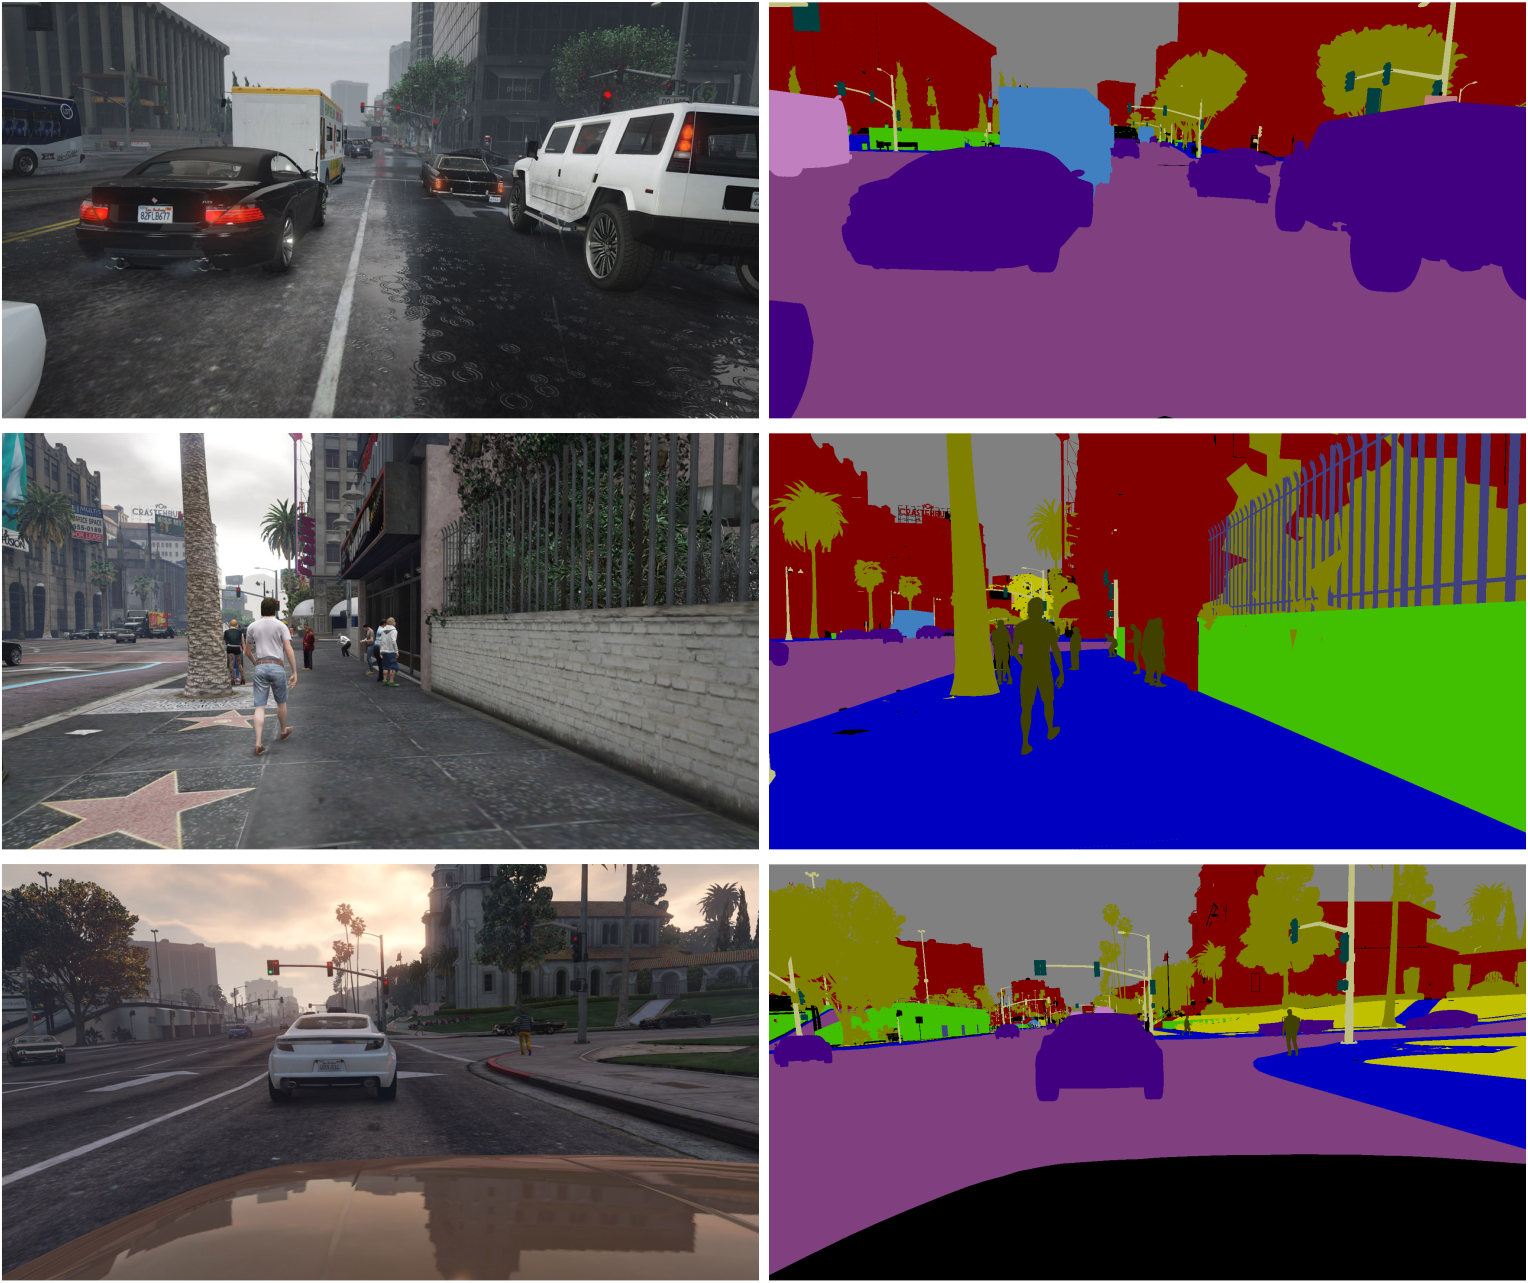
\includegraphics[width=\textwidth]{images/p4d_example.png}
	\caption{Example images (left) and corresponding ground-truth semantic label maps (right) provided in the GTA5 dataset \cite{Richter_2016_ECCV}.}
	\label{fig:p4d_examples}
\end{figure}

\newpage

\subsection{Real dataset:\\
	The Cityscapes Dataset for Semantic Urban Scene Understanding}

The Cityscapes dataset \cite{Cordts_2016_CVPR} is a large scale dataset containing car dashcam view images from 50 european cities. It includes 30 classes relevant for autonomous driving. The images include scenes in spring, summer and fall seasons and under different weather conditions. There are 5000 images provided together with fine annotations and 20000 together with coarse annotations. Due to the large amount of labeled data from a dashcam view and the inclusion of scenes with different weather and lighting conditions this dataset is often used to train deep neural networks that are related to autonomous driving. Due to the popularity and the GTA5 dataset containing compatible label maps, this work uses Cityscapes as the real dataset for the experiments. See Figure \ref{fig:cityscapes_examples} for Example images.

\begin{figure}
	\centering
	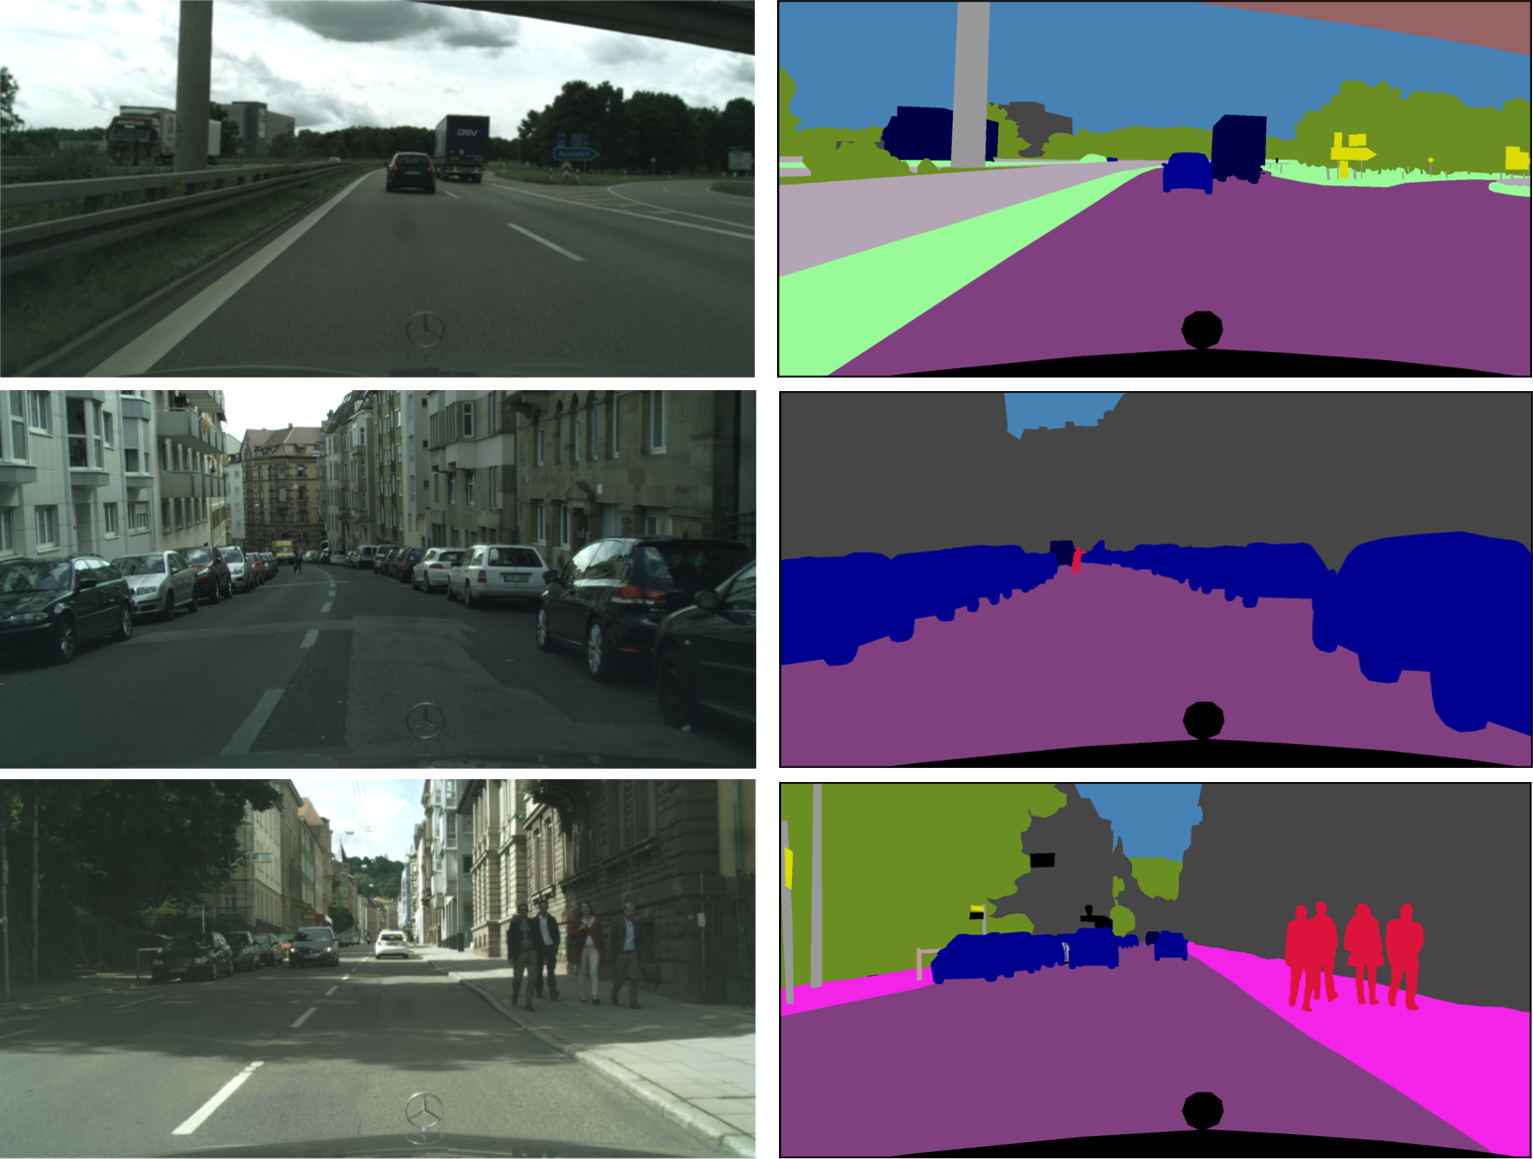
\includegraphics[width=\textwidth]{images/cityscapes_example.png}
	\caption{Example images (left) and corresponding ground-truth semantic label maps (right) provided in the Cityscapes dataset \cite{Cordts_2016_CVPR}.}
	\label{fig:cityscapes_examples}
\end{figure}

\section{Comparison Benchmark}
\subsection{Semantic Segmentation}
As this work is focused on datasets containing driving scenes the methods compared are applied to images that will then be performed semantic segmentation on. For the comparison Intersection over Union (IoU) is used. Intersection over Union is a metric often used to compare semantic segmentation methods' performance. All of the compared techniques were evaluated using IoU. It follows the following formula:
\begin{align*}
	\frac{\text{predicted pixels} \cap \text{ground truth pixels}}{\text{predicted pixels} \cup \text{ground truth pixels}}
\end{align*}
where predicted pixels are the pixels predicted for a specific class by the semantic segmentation model and ground truth pixels are the pixels containing the ground truth for that image. Usually, there are multiple different classes to predict and therefore it is common to calculate the mean IoU (mIoU) over all images that have predictions. To compare how well classes themselves are predicted by a model, one can also calculate the class IoU (cIoU).

\section{Methodology}
For the comparison each technique was used to translate a sample of 500 images from the GTA dataset to the Cityscapes domain. For CycleGAN and SG-GAN each, the authors provided pre-trained models. For CyCADA pretranslated images are provided in the project repository \cite{CyCADA}. To translate images with SG-GAN and CycleGAN the code provided in the repositories \cite{SG} and \cite{Cycle} was used. For the semantic segmentation task an implementation \cite{DLR} of DeepLabv3 \cite{DBLP:journals/corr/ChenPSA17} was used. To compute the IoU values the DeepLabv3 implementation uses the benchmark code provided by Cityscapes \cite{CSR}. All computations were run on a machine with Ubuntu 18.04 using an NVIDIA Geforce GTX 1070 with 8GB RAM. The images were scaled down to $512 \times 256$ pixels due to memory limitations while computing the CycleGAN samples.

\newpage

\section{Results}

\subsection{Quantitative}
As seen in Table \ref{table:results_quant}, CyCADA is the only method that improved average values for category and class semantic segmentation of the DeepLabv3 model. CyCADA improved the performance on per category average compared to untranslated GTA data by $2.2\%$ points, CycleGAN decreased it by $2\%$ points and SG-GAN by $4.2\%$ points. While SG-GAN was only able to improve the ``nature'' category and CycleGAN additionaly improved flat as well, CyCADA was able to improve 4 of the 7 categories tested. For per class average values, CycleGAN and SG-GAN decreased performance by $2.6\%$ points and $1.1\&$ point, respectively while CyCADA improved it by $1.6\%$ points. For the per class comparison, CycleGAN improved performance for 7 of the 19 tested classes compared to untranslated GTA5. SG-GAN was able to improve the scores for 8 out of 19 classes while having the best values for ``bus'', ``building'', ``traffic sign'' and ``vegetation''. CyCADA improves performance for 10 classes while performing approximately the same as untranslated GTA images for ``vegetation''. It holds the top values for ``building'', ``fence'', ``motorcycle'', ``road'', ``terrain'', ``train'', ``truck'' and ``wall''. The biggest improvement for CyCADA is category ``train'' where it improves semantic segmentation accuracy by $25.5\%$ points compared to GTA. See Table \ref{table:train} for an example that showcases the superior performance of semantic segmentation on the CyCADA translated image for the train category.

\begin{table}
	\centering
	\begin{tabular}{cc||c}
		\rotatebox[origin=c]{90}{\thead{GTA \\ (Ground Truth)}} & 
		\begin{minipage}[c]{0.45\textwidth}
			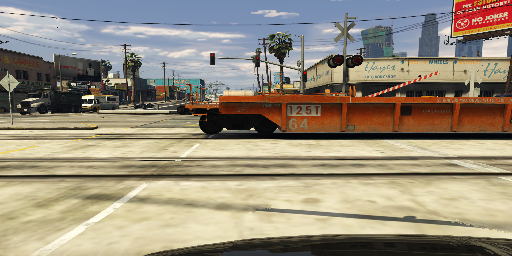
\includegraphics[width=\textwidth]{images/evaluation/GTA_gt_image_train.png}
		\end{minipage} & 
		\begin{minipage}[c]{0.45\textwidth}
			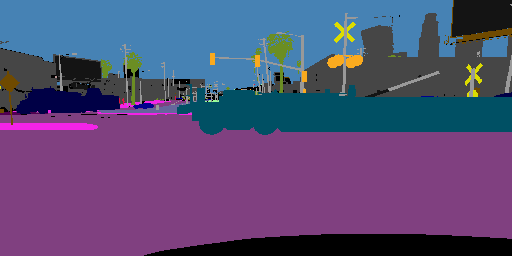
\includegraphics[width=\textwidth]{images/evaluation/GTA_gt_label_train.png}
		\end{minipage}\\
		\hline
		\hline
		\rotatebox[origin=c]{90}{GTA} &
		\multicolumn{1}{c||}{} &
		\begin{minipage}[c]{0.45\textwidth}
			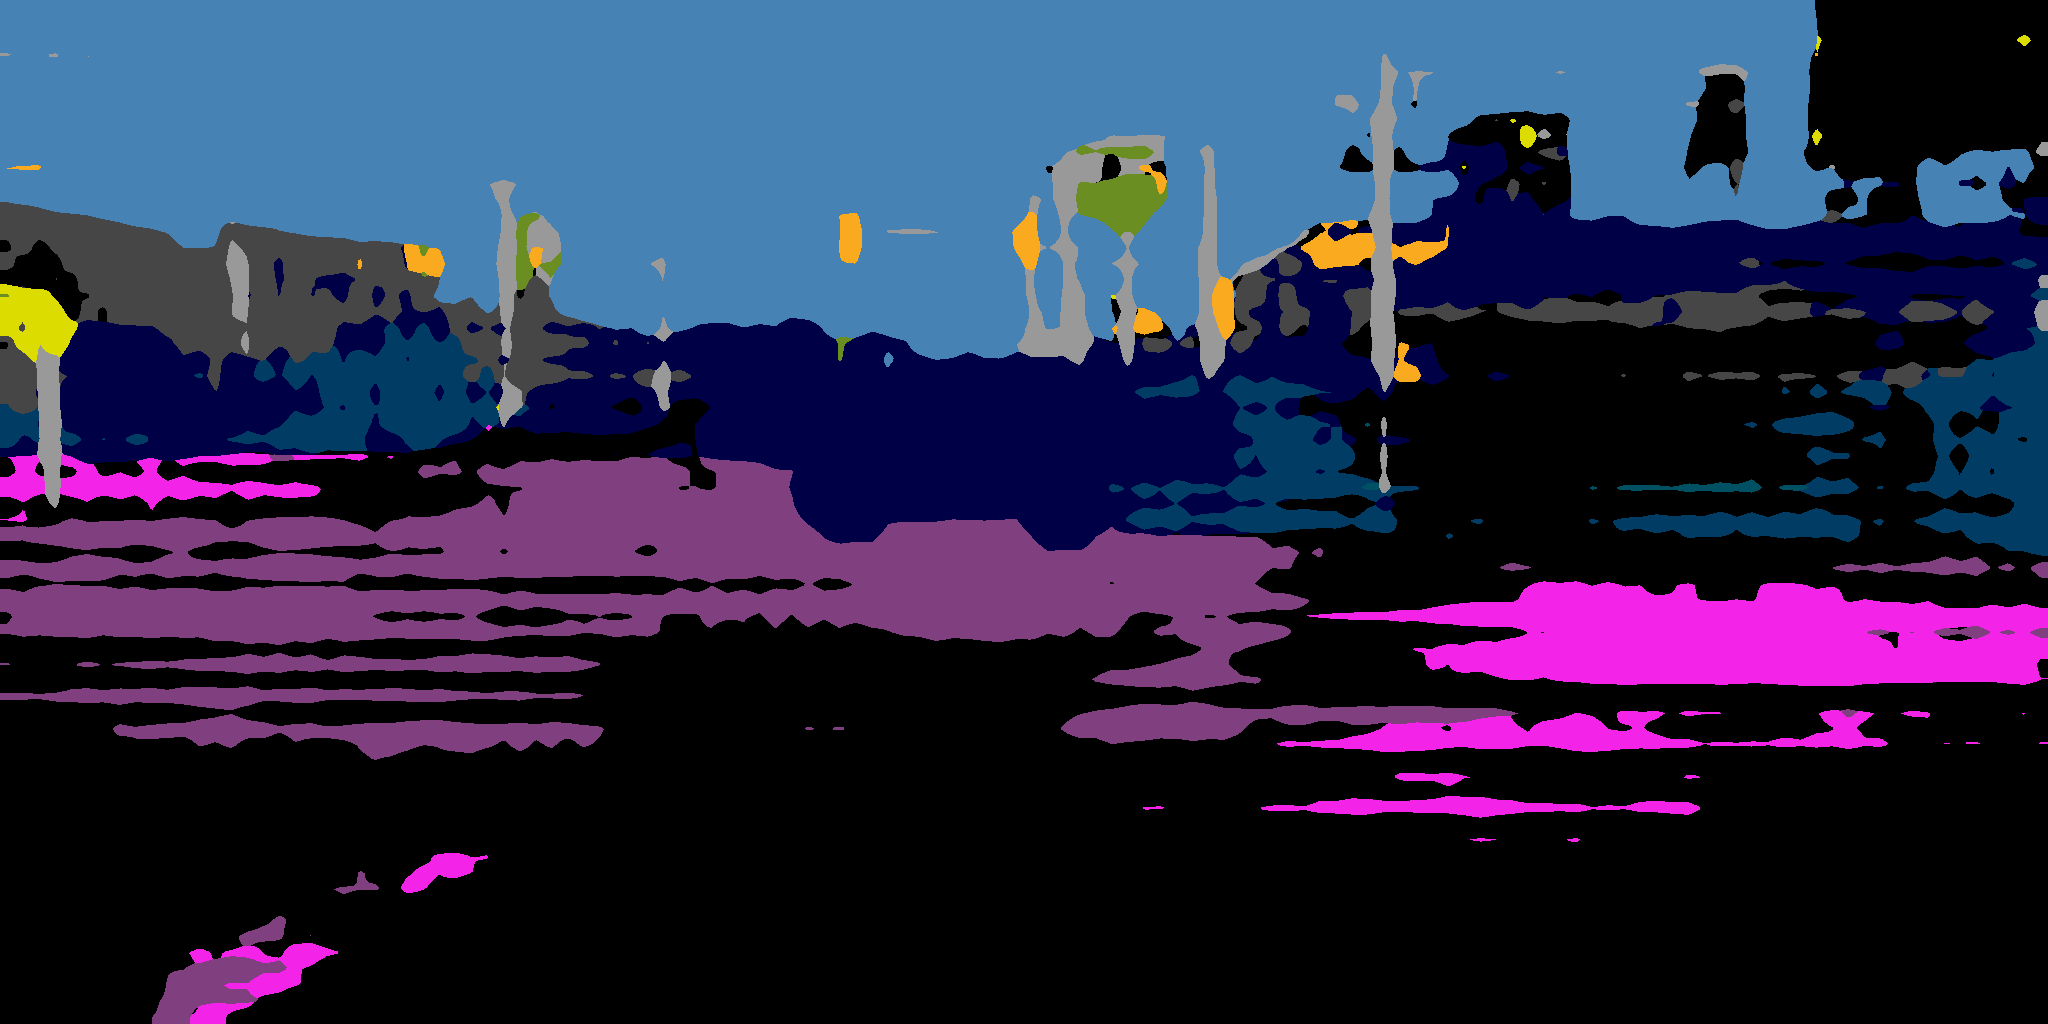
\includegraphics[width=\textwidth]{images/evaluation/GTA_pred_labels_train.png}
		\end{minipage}\\
		\rotatebox[origin=c]{90}{CycleGAN} &
		\begin{minipage}[c]{0.45\textwidth}
			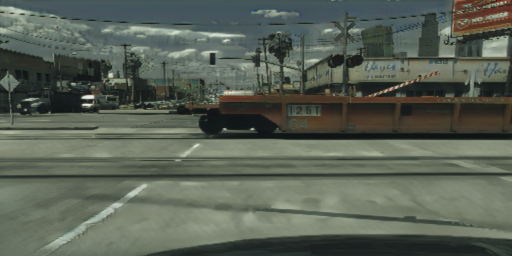
\includegraphics[width=\textwidth]{images/evaluation/CycleGAN_translated_train.png}
		\end{minipage} &
		\begin{minipage}[c]{0.45\textwidth}
			
\includegraphics[width=\textwidth]{images/evaluation/CycleGAN_pred_labels_train.png}
		\end{minipage}\\
		\rotatebox[origin=c]{90}{CyCADA} &
		\begin{minipage}[c]{0.45\textwidth} 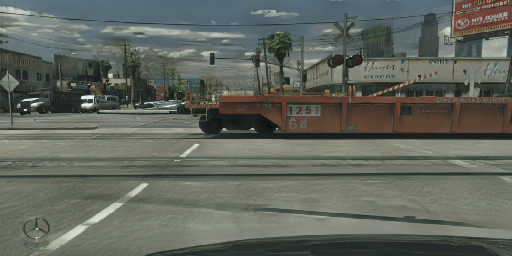
\includegraphics[width=\textwidth]{images/evaluation/CyCADA_translated_train.png} 
		\end{minipage}& 
		\begin{minipage}[c]{0.45\textwidth}
			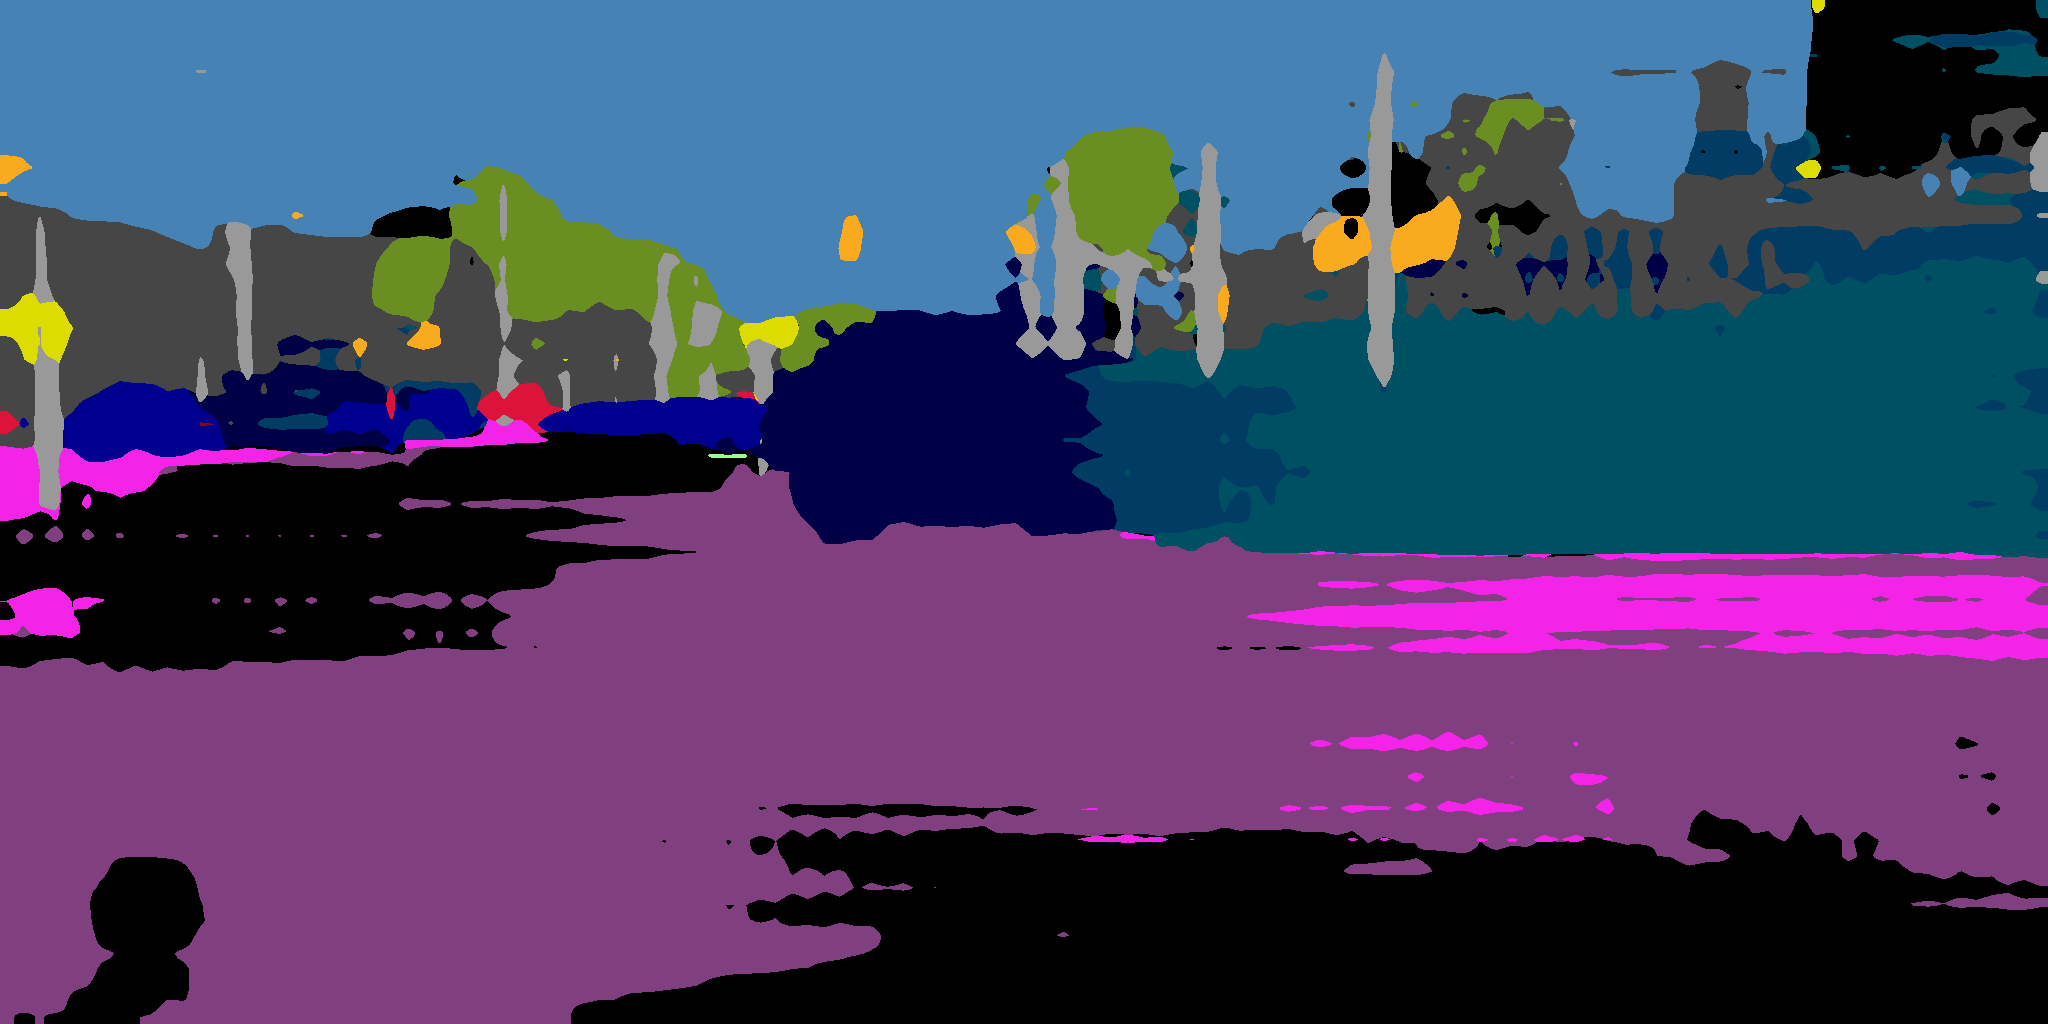
\includegraphics[width=\textwidth]{images/evaluation/CyCADA_pred_labels_train.png}
		\end{minipage}\\
		\rotatebox[origin=c]{90}{SG-GAN} &
		\begin{minipage}[c]{0.45\textwidth} 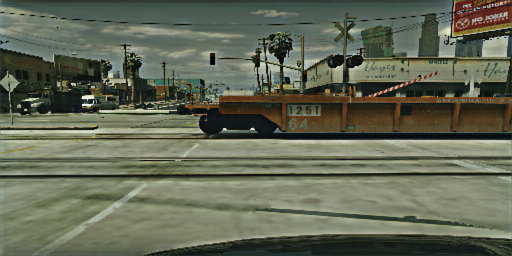
\includegraphics[width=\textwidth]{images/evaluation/SG-GAN_translated_train.png}
		\end{minipage} & 
		\begin{minipage}[c]{0.45\textwidth}
			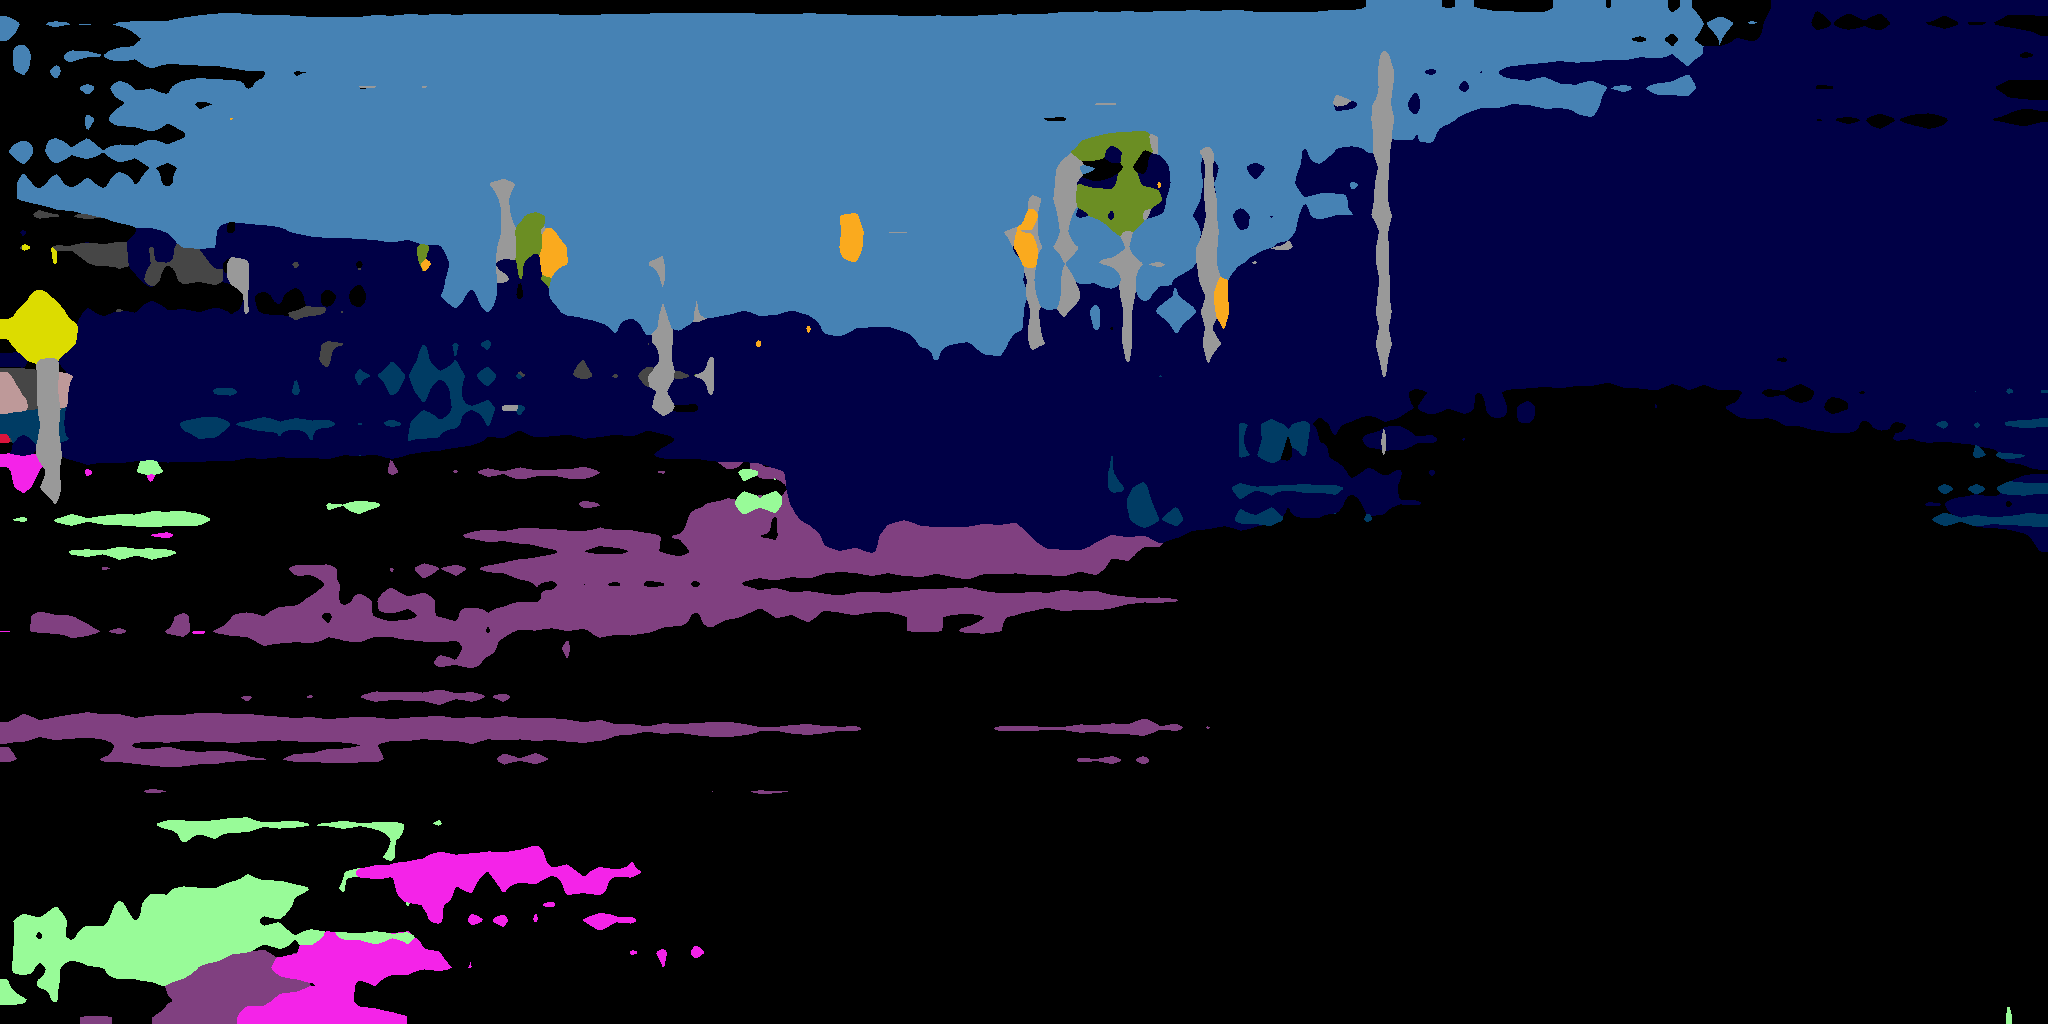
\includegraphics[width=\textwidth]{images/evaluation/SG-GAN_pred_labels_train.png}
		\end{minipage} \\
		%\multicolumn{2}{c}{} \\
		\multicolumn{1}{c}{} & (translated) Image & (predicted) Labelmap
	\end{tabular} 
	\caption{An example of an image containing a train. Comparing the images translated by the different methods and the corresponding semantic segmentation. It is easy to see that CyCADA performs best in this comparison on semantic segmentation of the train (colored dark teal).}
	\label{table:train}
\end{table}

\begin{table}
	\centering
	\begin{tabular}{|c|c|c|c|c|}
		\multicolumn{5}{c}{\textbf{category Scores}}\\
		\hline
		\multicolumn{1}{c}{} & \multicolumn{4}{c}{Methods}\\
		\cline{2-5}
		\multicolumn{1}{c|}{category} & GTA5 & CycleGAN & CyCADA & SG-GAN\\ 
		\hline
		construction & 0.636 & 0.598 & \textbf{0.674} & 0.628\\ 
		\hline 
		flat & 0.740 & 0.861 & \textbf{0.894} & 0.735\\ 
		\hline 
		human & \textbf{0.546} & 0.402 & 0.440 & 0.487\\ 
		\hline 
		nature & 0.543 & 0.615 & \textbf{0.622} & 0.585\\ 
		\hline 
		object & \textbf{0.085} & 0.067 & 0.073 & 0.080\\ 
		\hline 
		sky & \textbf{0.872} & 0.822 & 0.832 & 0.644\\ 
		\hline 
		vehicle & 0.641 & 0.557 & \textbf{0.680} & 0.609\\ 
		\hline \hline
		average & 0.580 & 0.560 & \textbf{0.602} & 0.538\\
		\hline
		\multicolumn{5}{c}{}\\
		\multicolumn{5}{c}{\textbf{class Scores}}\\
		\hline
		\multicolumn{1}{c}{} & \multicolumn{4}{c}{Methods}\\
		\cline{2-5}
		\multicolumn{1}{c|}{class} & GTA5 & CycleGAN & CyCADA & SG-GAN\\ 
		\hline
		bicycle & \textbf{0.100} & 0.038 & 0.041 & 0.051\\ 
		\hline 
		building & 0.620 & 0.509 & \textbf{0.634} & 0.513\\ 
		\hline 
		bus & 0.209 & 0.136 & 0.190 & \textbf{0.257}\\ 
		\hline 
		car & 0.627 & 0.570 & 0.640 & \textbf{0.642}\\ 
		\hline 
		fence & 0.100 & 0.102 & \textbf{0.125} & 0.083\\ 
		\hline 
		motorcycle & 0.195 & 0.125 & \textbf{0.297} & 0.256\\ 
		\hline 
		person & \textbf{0.524} & 0.369 & 0.398 & 0.461\\ 
		\hline 
		pole & 0.0 & 0.0 & 0.0 & 0.0\\ 
		\hline 
		rider & \textbf{0.312} & 0.160 & 0.144 & 0.247\\ 
		\hline 
		road & 0.658 & 0.752 & \textbf{0.775} & 0.631\\ 
		\hline 
		sidewalk & \textbf{0.434} & 0.365 & 0.339 & 0.381\\ 
		\hline 
		sky & \textbf{0.872} & 0.822 & 0.832 & 0.644\\ 
		\hline 
		terrain & 0.282 & 0.361 & \textbf{0.374} & 0.292\\ 
		\hline 
		traffic light & \textbf{0.210} & 0.178 & 0.187 & 0.185\\ 
		\hline 
		traffic sign & 0.090 & 0.126 & 0.120 & \textbf{0.158}\\ 
		\hline 
		train & 0.025 & 0.115 & \textbf{0.280} & 0.222\\ 
		\hline 
		truck & 0.387 & 0.371 & \textbf{0.511} & 0.332\\ 
		\hline 
		vegetation & 0.595 & 0.620 & 0.595 & \textbf{0.653}\\ 
		\hline 
		wall & 0.162 & 0.186 & \textbf{0.225} & 0.186\\ 
		\hline \hline 
		average & 0.337 & 0.311 & \textbf{0.353} & 0.326\\
		\hline
	\end{tabular} 
	\caption{Intersection over Union results for evaluation on untranslated GTA5 images and translated images by CycleGAN, CyCADA and SG-GAN respectively. Rounded to 3 decimal places. Maximum value per row is written in big font.}
	\label{table:results_quant}
\end{table}

\subsection{Qualitative}
Table \ref{table:results_qual} shows a qualitative comparison for a single frame translated through each method and with corresponding predicted labelmap. One can see that all of the techniques darkened the overall appearance of the image while SG-GAN still has brighter color than CycleGAN and CyCADA. CyCADA smooths out the road the most out of all of the techniques and SG-GAN least. SG-GAN has a lot of noisy structure in the translated images. Also they have a bright glow between the sky and other semantic classes. The only technique that learned the mercedes star and generates it in most of the images is CyCADA. Overall, the SG-GAN images look very sharp and close to the original GTA images while CycleGAN and CyCADA smooth out the textures more. The pedestrians on the right side of the images are more clearly generated in CyCADA than CycleGAN. The predicted labelmap of the ground truth GTA image clearly shows that the DeepLabv3 model trained on Cityscapes performs worse in the synthetic domain. For SG-GAN it predicts large portions of the road as sidewalks and generates noisy label images. The DeepLabv3 model is able to successfully predict streets and sidewalks for CyCADA and CycleGAN images. While it predicts some regions other than the ego car as void for SG-GAN and CycleGAN, CyCADA only has one small region that it cannot predict as belonging to one of the main classes. The CyCADA label map contains more vegetation than the ground truth. 

% void
\definecolor{black}{rgb}{0, 0, 0} % unlabeled, ego vehicle, rectification border, out of roi, static

%flat
\definecolor{purple}{rgb}{0.5, 0.25, 0.5} %road
\definecolor{lightpurple}{rgb}{0.96, 0.14, 0.91} %sidewalk

% construction
\definecolor{grey}{rgb}{0.27, 0.27, 0.27} % building
\definecolor{bluepurple}{rgb}{0.4, 0.4, 0.61} % wall
\definecolor{darkerskin}{rgb}{0.75, 0.6, 0.6} % fence

%object
\definecolor{grey2}{rgb}{0.6, 0.6, 0.6} % pole
\definecolor{orange}{rgb}{0.98, 0.67, 0.12} % traffic light
\definecolor{lightgreen}{rgb}{0.86, 0.86, 0} % traffic sign

%nature
\definecolor{green}{rgb}{0.42, 0.56, 0.14} % vegetation
\definecolor{brightgreen}{rgb}{0.60, 0.98, 0.60} % terrain

%sky
\definecolor{blue}{rgb}{0.27, 0.51, 0.71} % sky

%human
\definecolor{red}{rgb}{0.86, 0.08, 0.24} % person
\definecolor{fullred}{rgb}{1, 0, 0} % rider

%vehicle
\definecolor{darkblue}{rgb}{0, 0, 0.56} % car
\definecolor{blueblack}{rgb}{0, 0, 0.27} % truck
\definecolor{paleblue}{rgb}{0, 0.24, 0.39} % bus
\definecolor{palegreenblue}{rgb}{0, 0.31, 0.39} % train
\definecolor{brightblue}{rgb}{0, 0, 0.90} % motorcycle
\definecolor{brownred}{rgb}{0.47, 0.04, 0.13} % bicycle

\begin{table}
	\centering
	\setlength\tabcolsep{1.5pt}
%	\begin{tabular}{cc||c}
%		\rotatebox[origin=c]{90}{\thead{GTA \\ (Ground Truth)}} & 
%		\begin{minipage}[c]{0.45\textwidth}
%			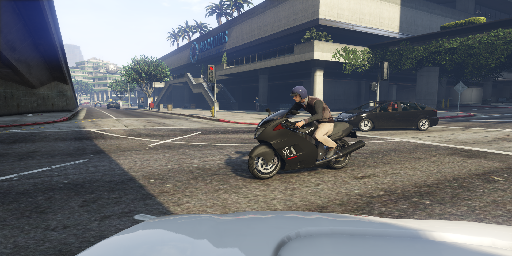
\includegraphics[width=\textwidth]{images/evaluation/00991_leftImg8bit.png}
%		\end{minipage} & 
%		\begin{minipage}[c]{0.45\textwidth}
%			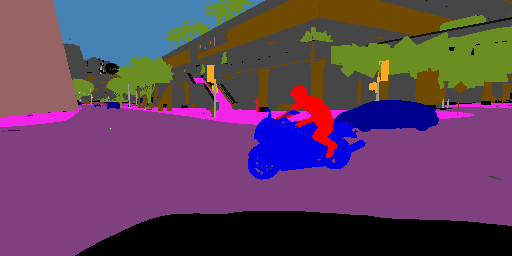
\includegraphics[width=\textwidth]{images/evaluation/00991_gtFine_labelIds.png}
%		\end{minipage}\\
%		\hline
%		\hline
%		\rotatebox[origin=c]{90}{GTA} &
%		\multicolumn{1}{c||}{} &
%		\begin{minipage}[c]{0.45\textwidth}
%			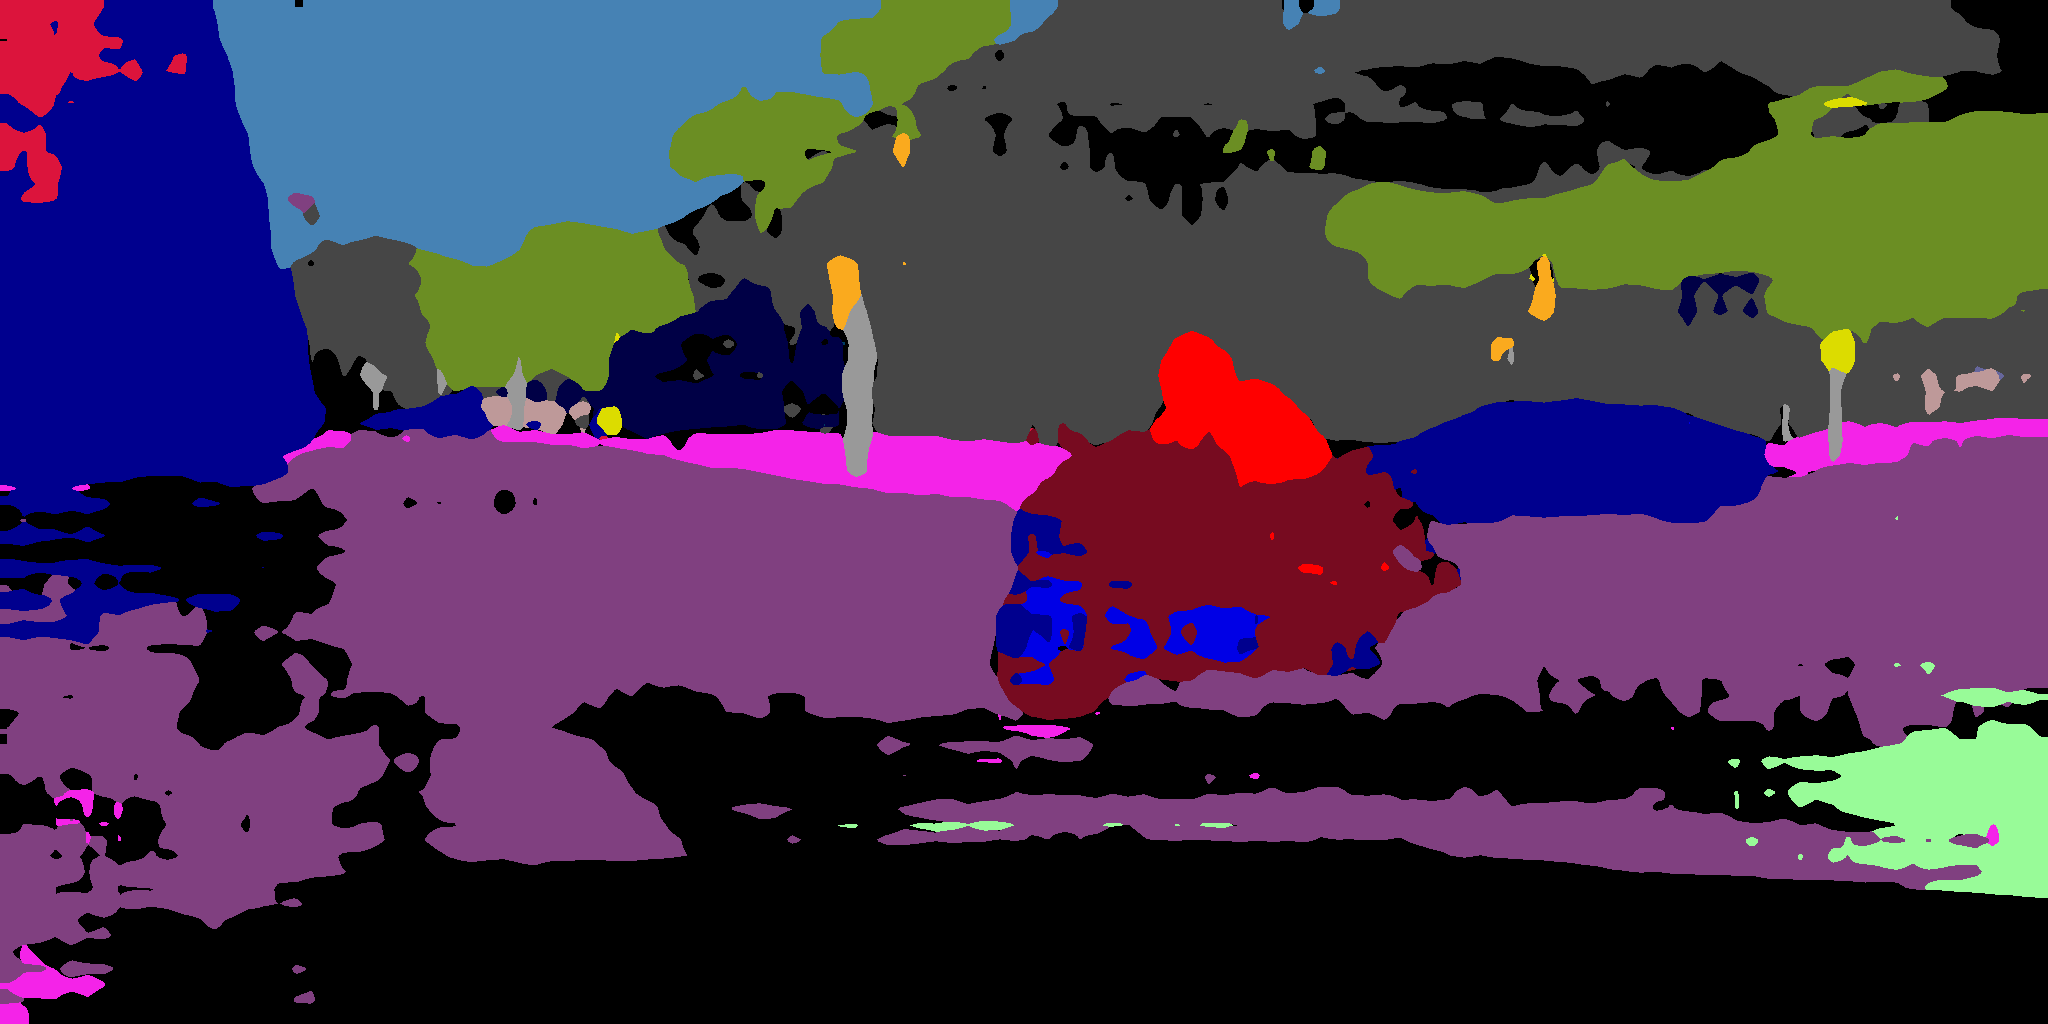
\includegraphics[width=\textwidth]{images/evaluation/gta_00991_pred_label_img.png}
%		\end{minipage}\\
%		\rotatebox[origin=c]{90}{CycleGAN} &
%		\begin{minipage}[c]{0.45\textwidth}
%			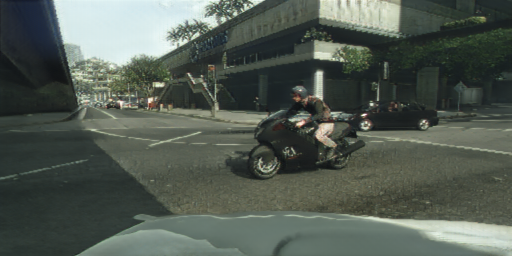
\includegraphics[width=\textwidth]{images/evaluation/CycleGAN_00991_leftImg8bit.png}
%		\end{minipage} &
%		\begin{minipage}[c]{0.45\textwidth}
%			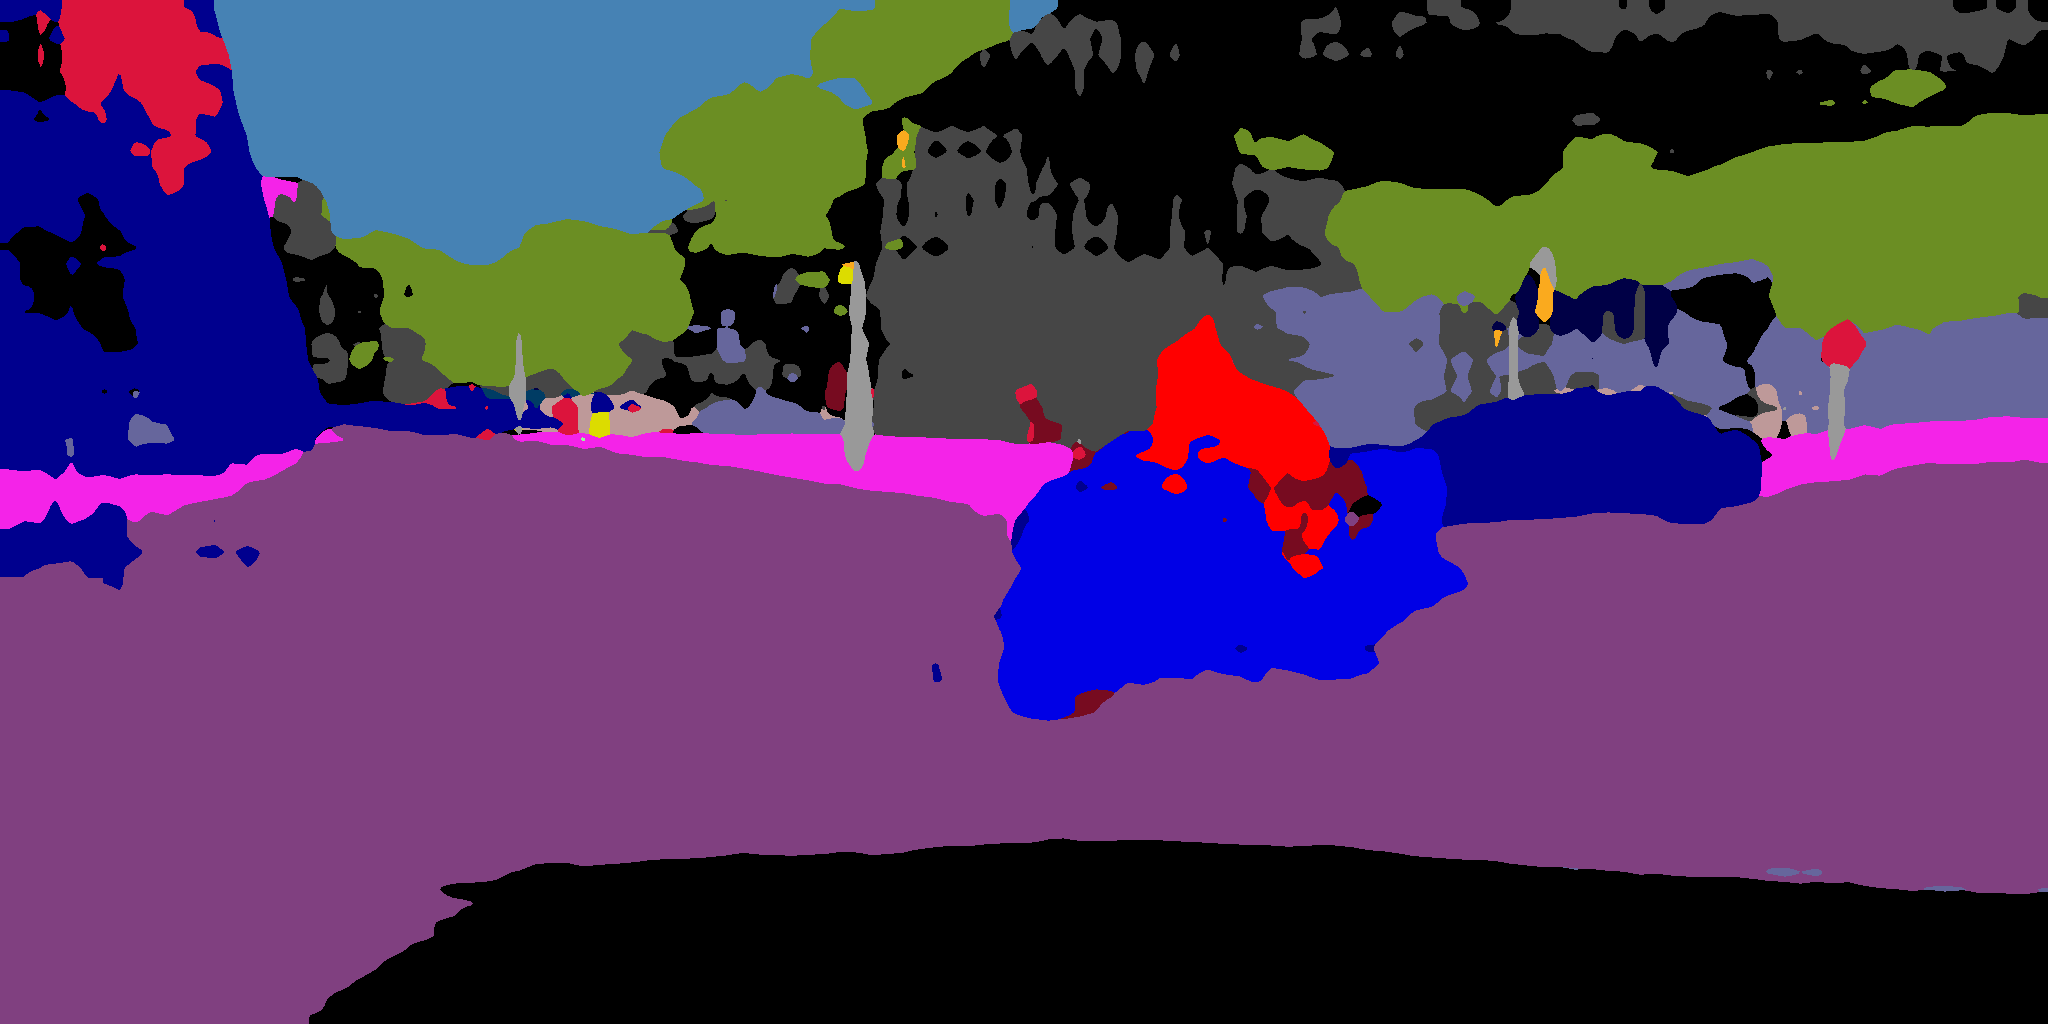
\includegraphics[width=\textwidth]{images/evaluation/CycleGAN_00991_pred_label_img.png}
%		\end{minipage}\\
%		\rotatebox[origin=c]{90}{CyCADA} &
%		\begin{minipage}[c]{0.45\textwidth} 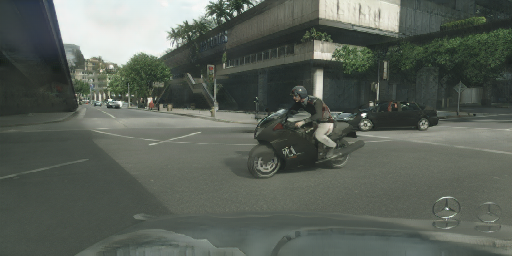
\includegraphics[width=\textwidth]{images/evaluation/CyCADA_00991_leftImg8bit.png} 
%		\end{minipage}& 
%		\begin{minipage}[c]{0.45\textwidth}
%			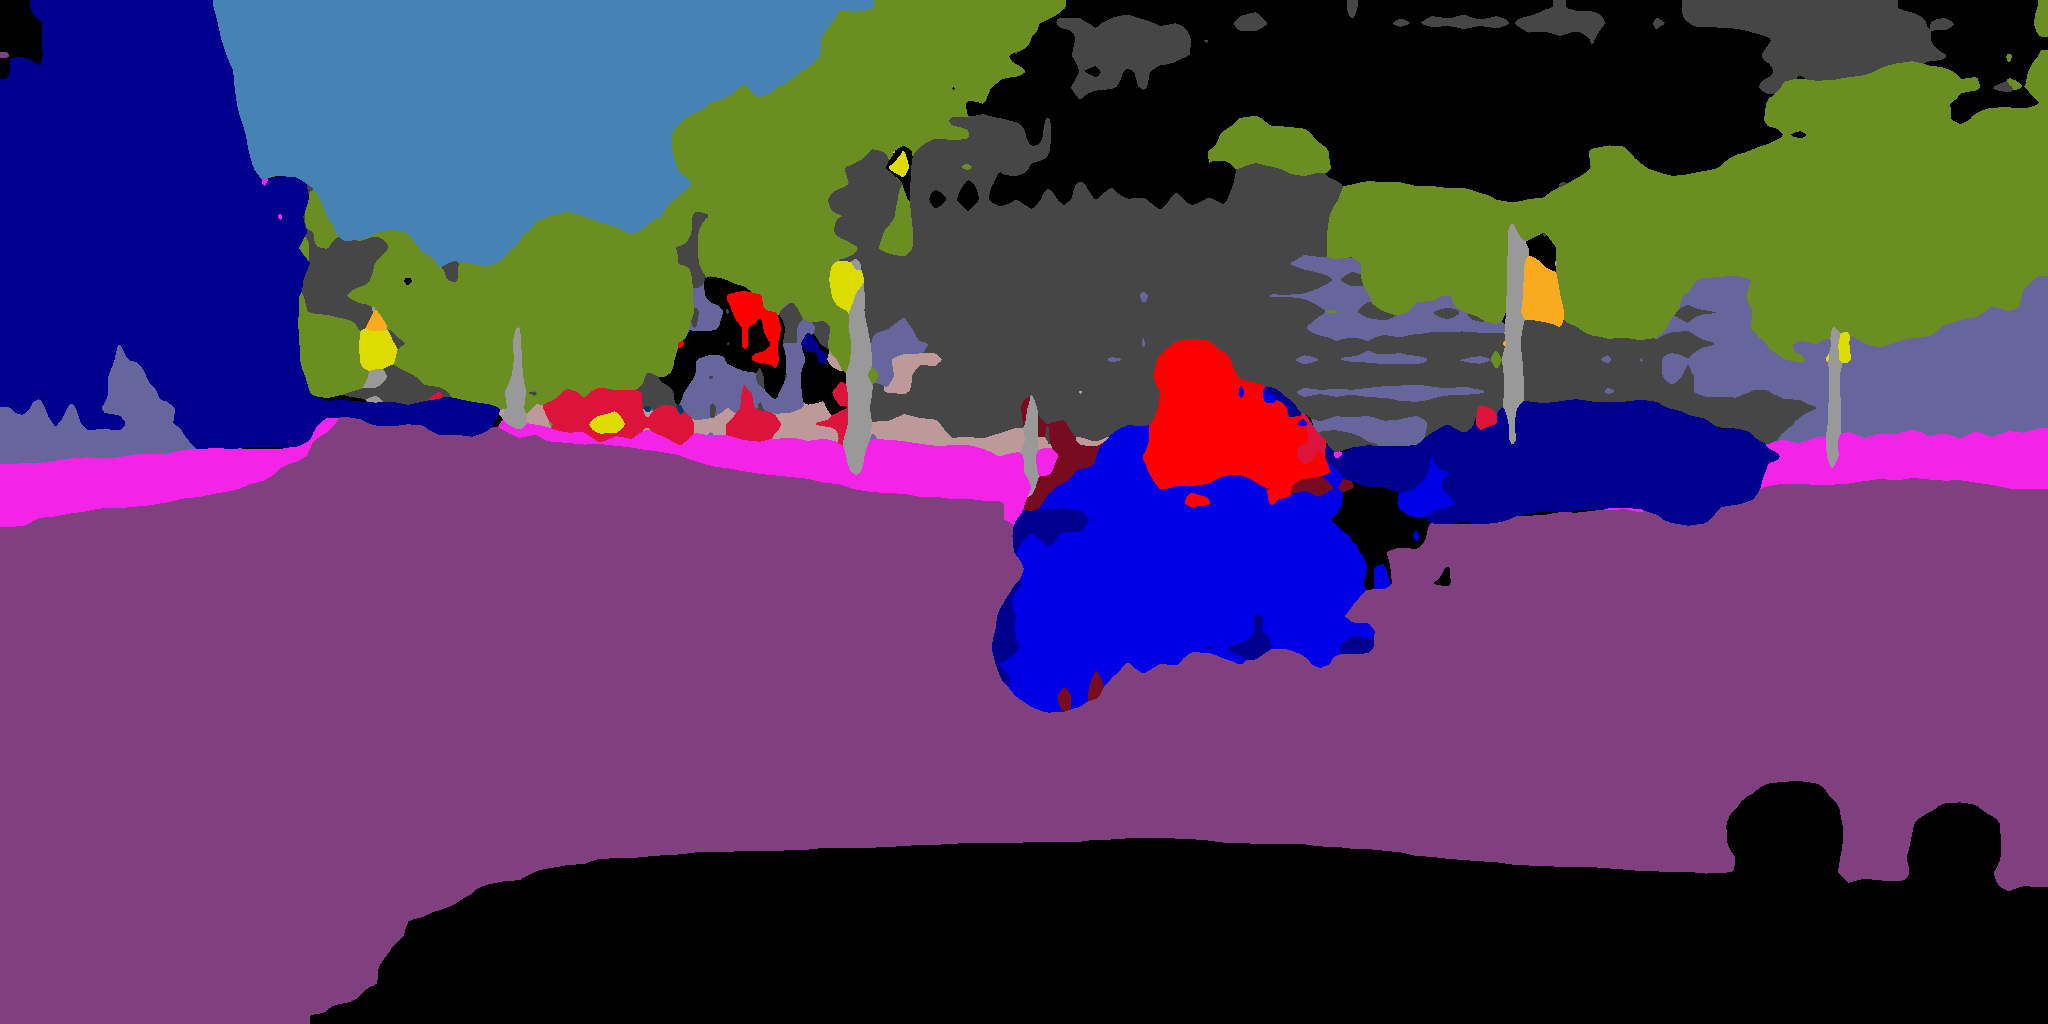
\includegraphics[width=\textwidth]{images/evaluation/CyCADA_00991_pred_label_img.png}
%		\end{minipage}\\
%		\rotatebox[origin=c]{90}{SG-GAN} &
%		\begin{minipage}[c]{0.45\textwidth} 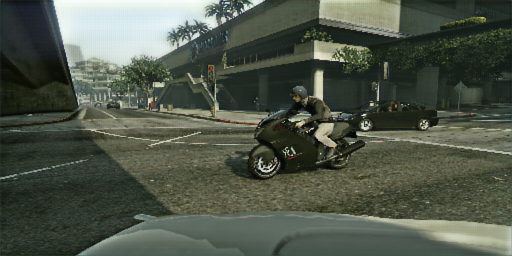
\includegraphics[width=\textwidth]{images/evaluation/SG-GAN_00991_leftImg8bit.png}
%		\end{minipage} & 
%		\begin{minipage}[c]{0.45\textwidth}
%			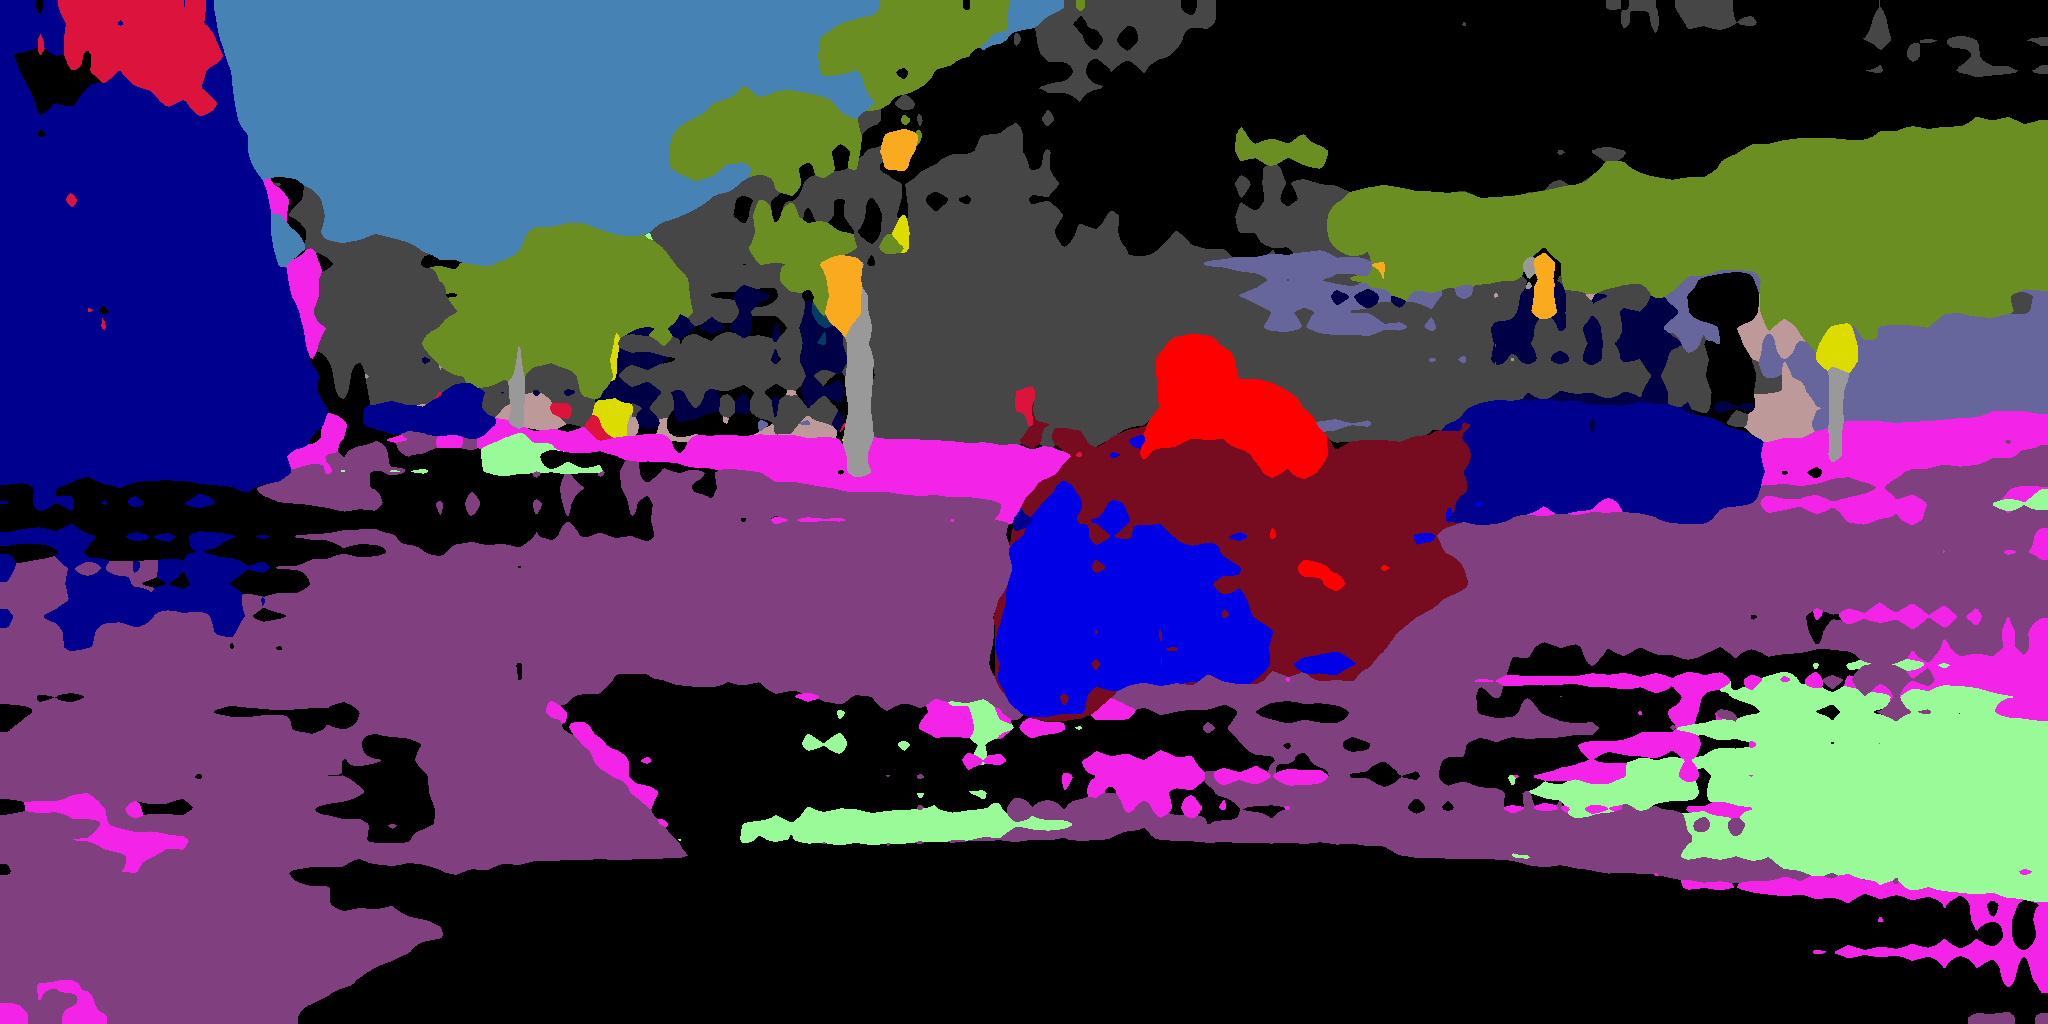
\includegraphics[width=\textwidth]{images/evaluation/SG-GAN_00991_pred_label_img.png}
%		\end{minipage} \\
%		%\multicolumn{2}{c}{} \\
%		\multicolumn{1}{c}{} & (translated) Image & (predicted) Labelmap
%	\end{tabular}
		\begin{tabular}{cc||c}
		\rotatebox[origin=c]{90}{\thead{GTA \\ (Ground Truth)}} & 
		\begin{minipage}[c]{0.45\textwidth}
			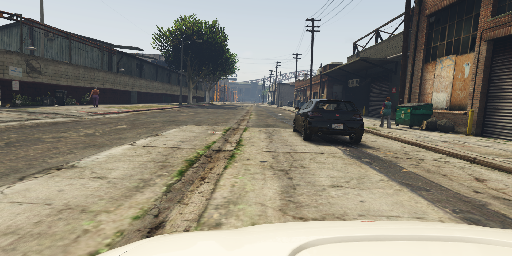
\includegraphics[width=\textwidth]{images/evaluation/GTA_gt_image.png}
		\end{minipage} & 
		\begin{minipage}[c]{0.45\textwidth}
			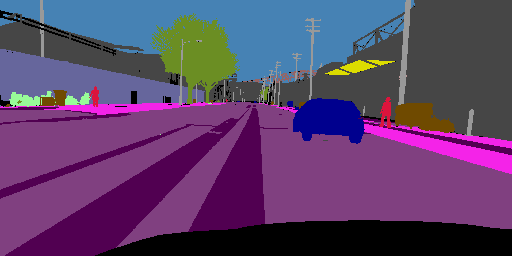
\includegraphics[width=\textwidth]{images/evaluation/GTA_gt_label.png}
		\end{minipage}\\
		\hline
		\hline
		\rotatebox[origin=c]{90}{GTA} &
		\multicolumn{1}{c||}{} &
		\begin{minipage}[c]{0.45\textwidth}
			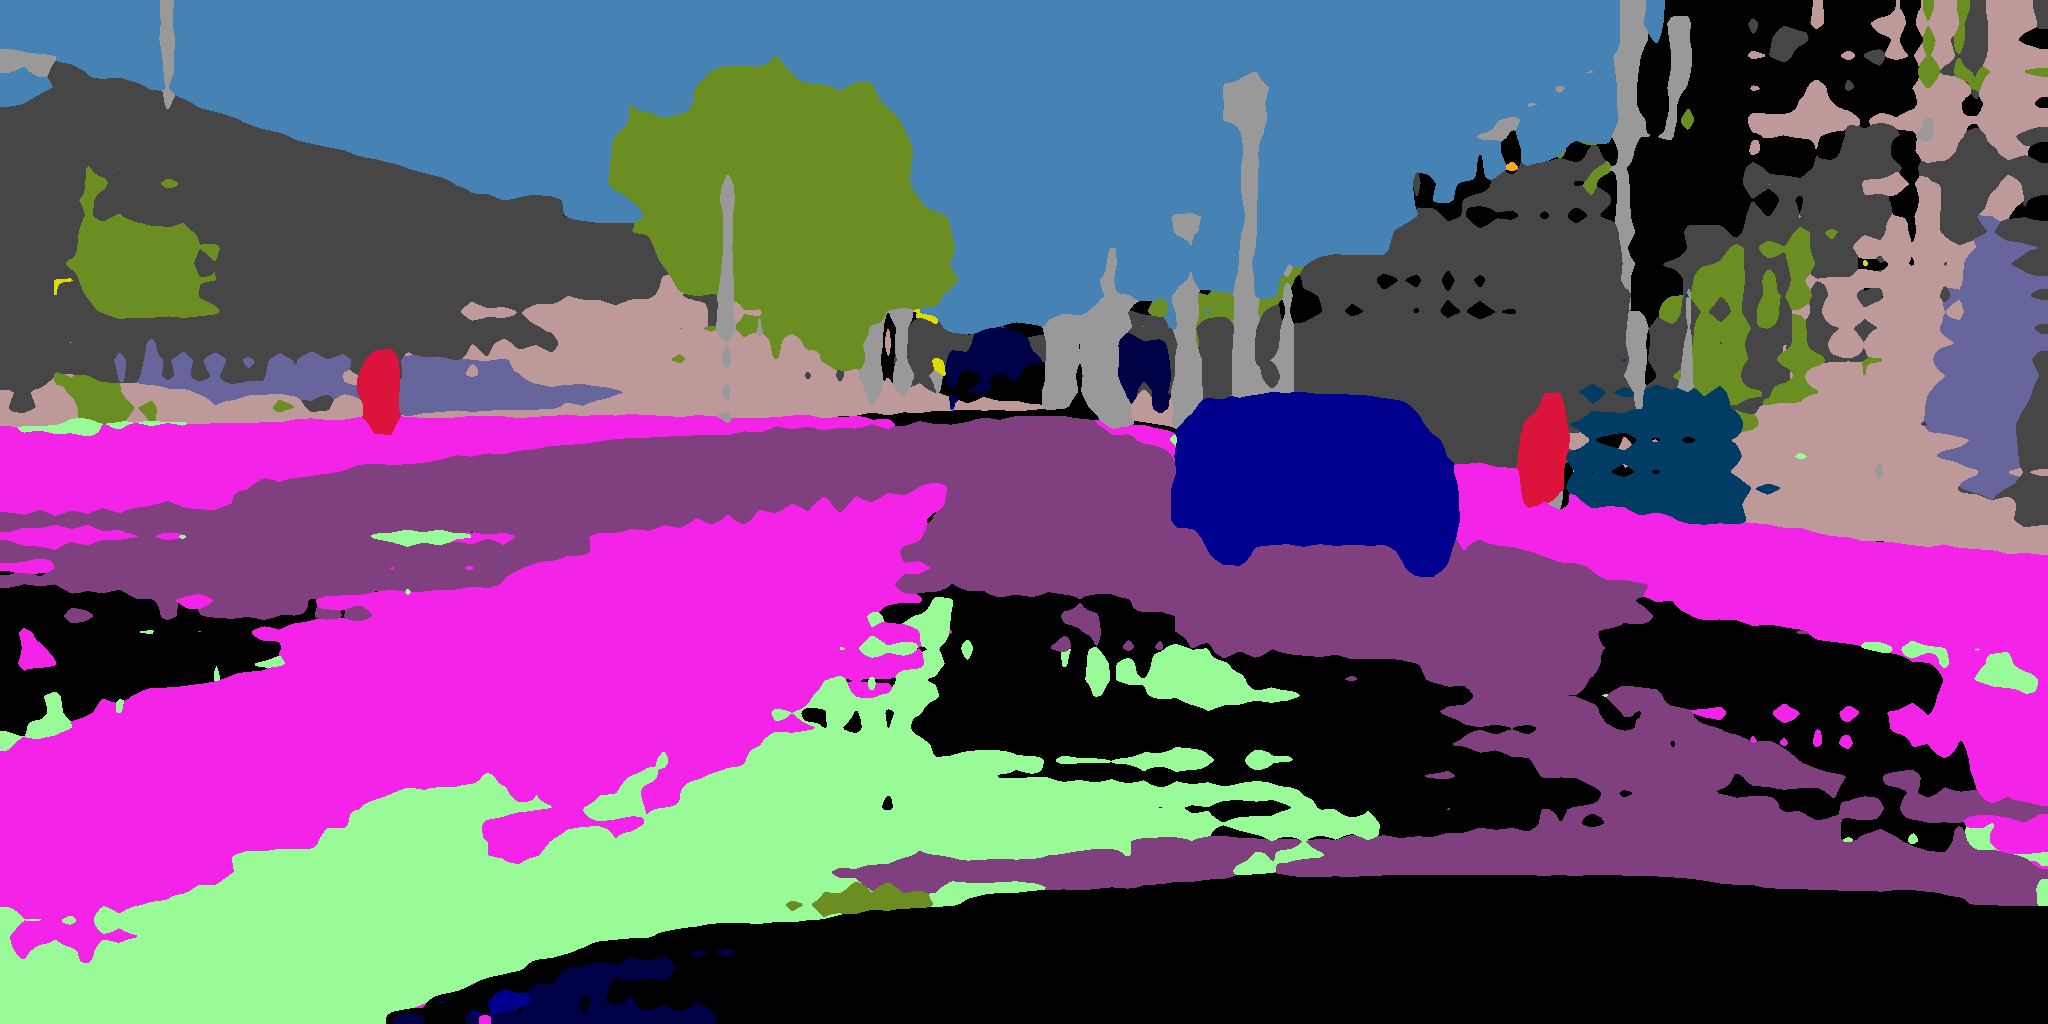
\includegraphics[width=\textwidth]{images/evaluation/GTA_pred_labels.png}
		\end{minipage}\\
		\rotatebox[origin=c]{90}{CycleGAN} &
		\begin{minipage}[c]{0.45\textwidth}
			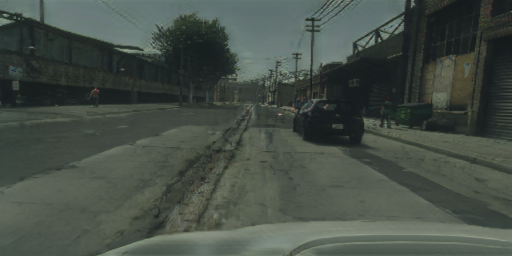
\includegraphics[width=\textwidth]{images/evaluation/CycleGAN_translated.png}
		\end{minipage} &
		\begin{minipage}[c]{0.45\textwidth}
			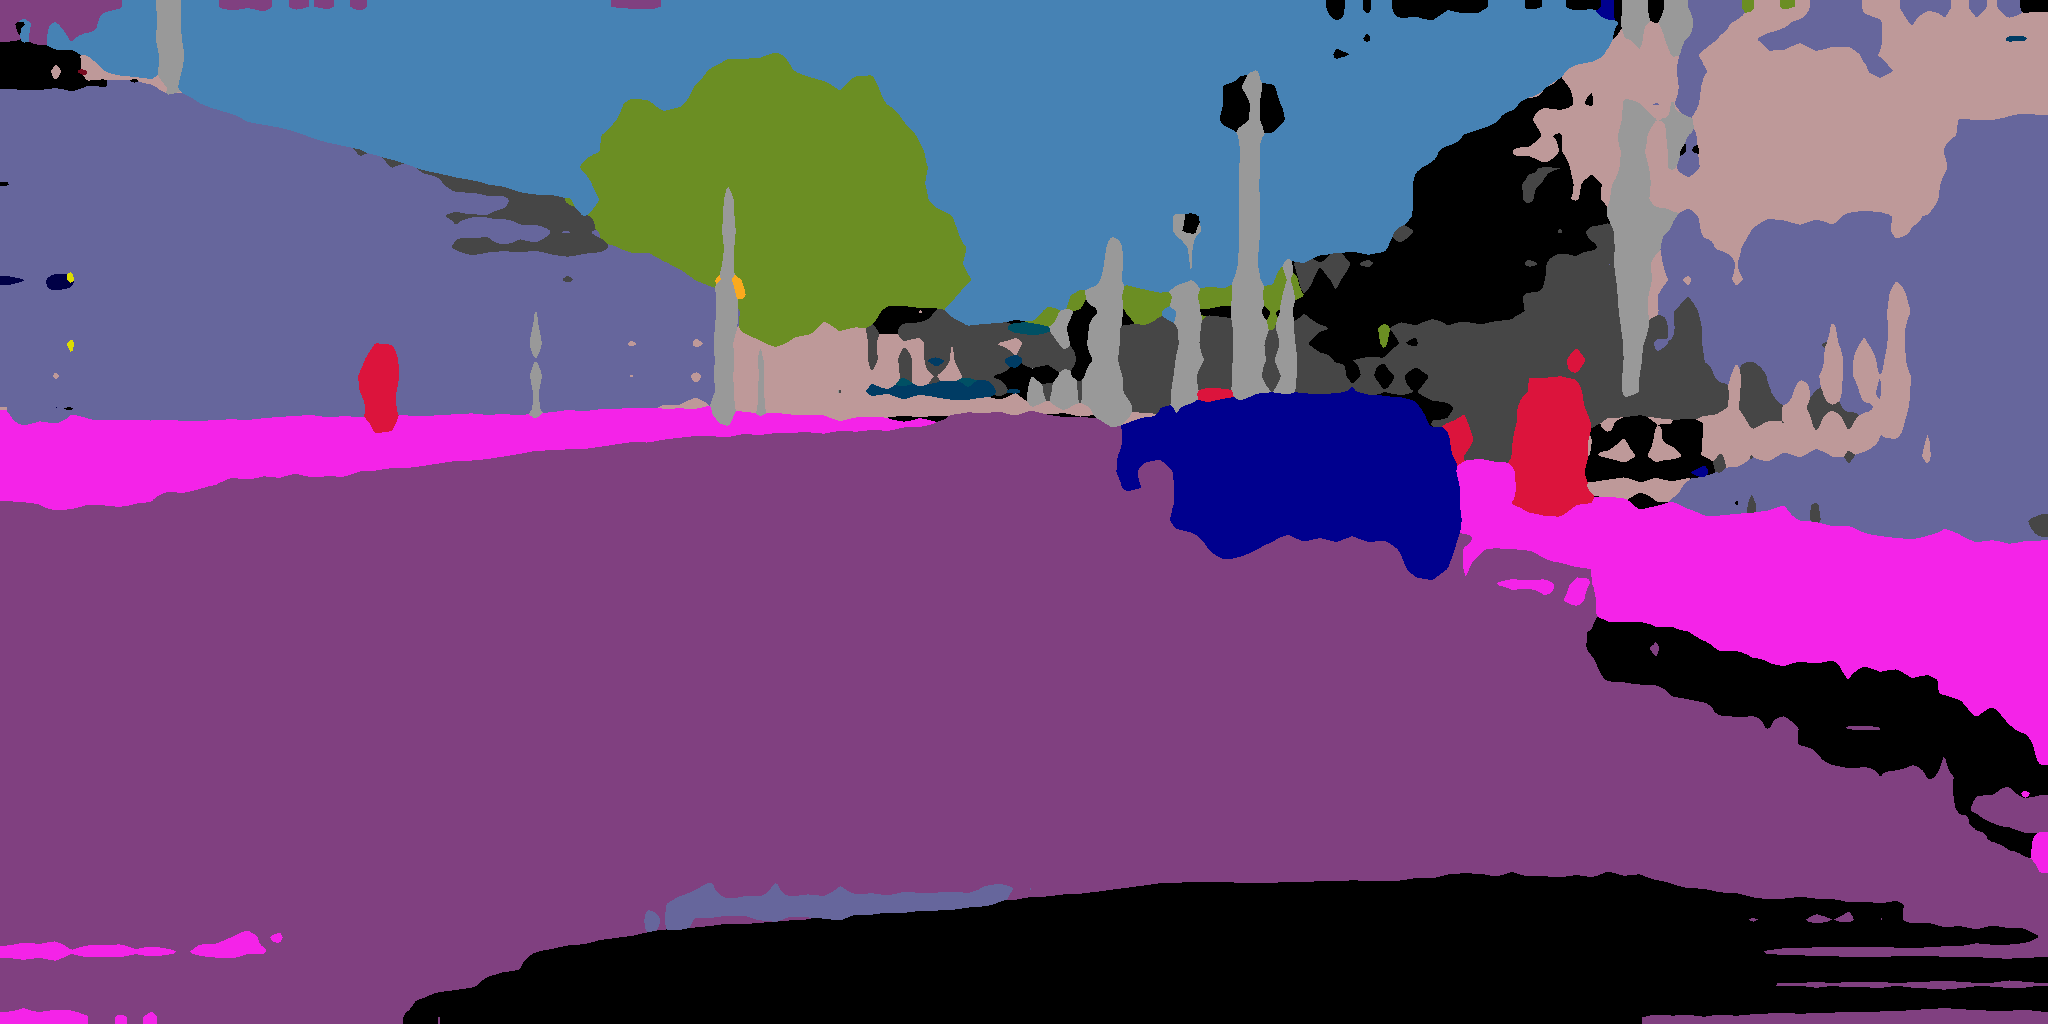
\includegraphics[width=\textwidth]{images/evaluation/CycleGAN_pred_labels.png}
		\end{minipage}\\
		\rotatebox[origin=c]{90}{CyCADA} &
		\begin{minipage}[c]{0.45\textwidth} 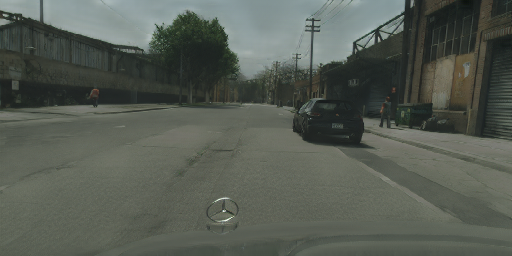
\includegraphics[width=\textwidth]{images/evaluation/CyCADA_translated.png} 
		\end{minipage}& 
		\begin{minipage}[c]{0.45\textwidth}
			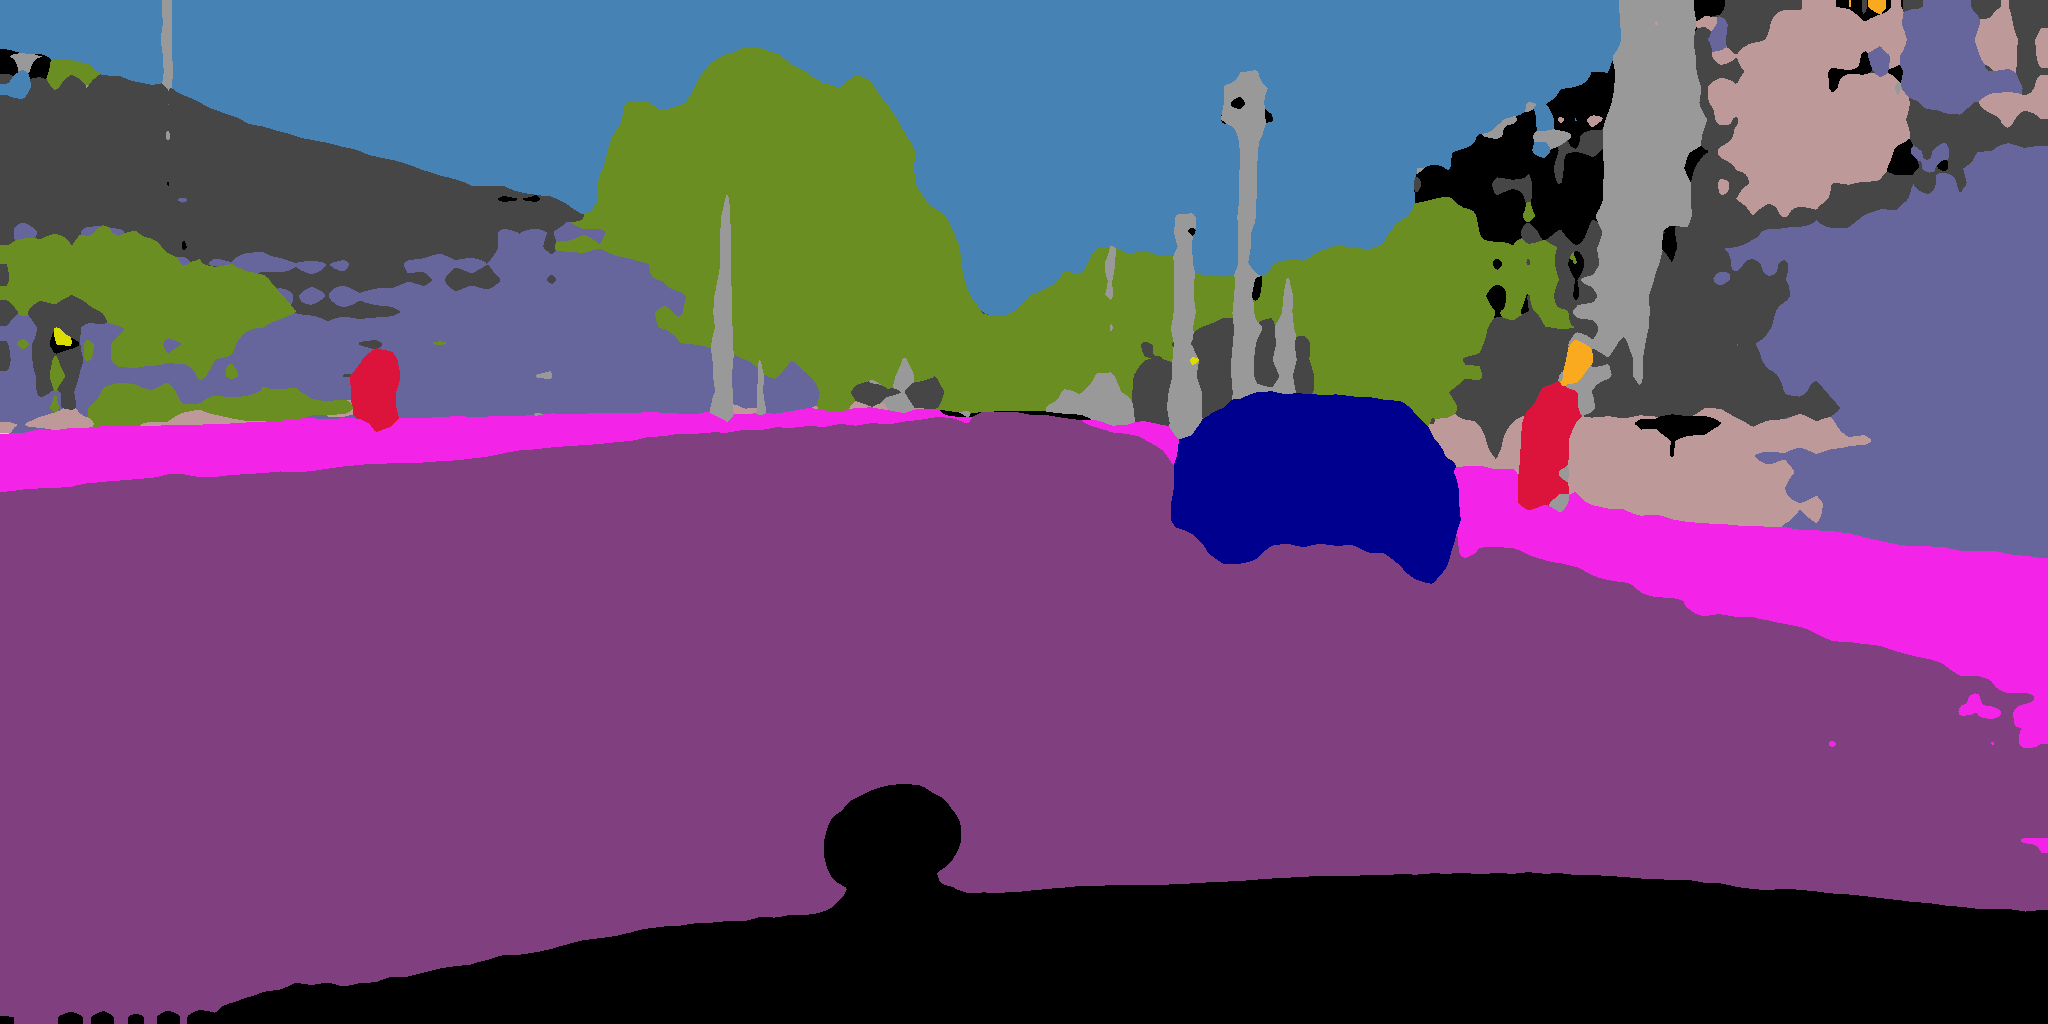
\includegraphics[width=\textwidth]{images/evaluation/CyCADA_pred_labels.png}
		\end{minipage}\\
		\rotatebox[origin=c]{90}{SG-GAN} &
		\begin{minipage}[c]{0.45\textwidth} 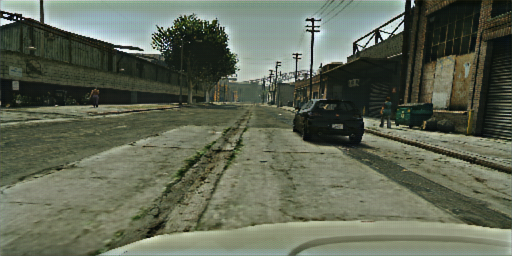
\includegraphics[width=\textwidth]{images/evaluation/SG-GAN_translated.png}
		\end{minipage} & 
		\begin{minipage}[c]{0.45\textwidth}
			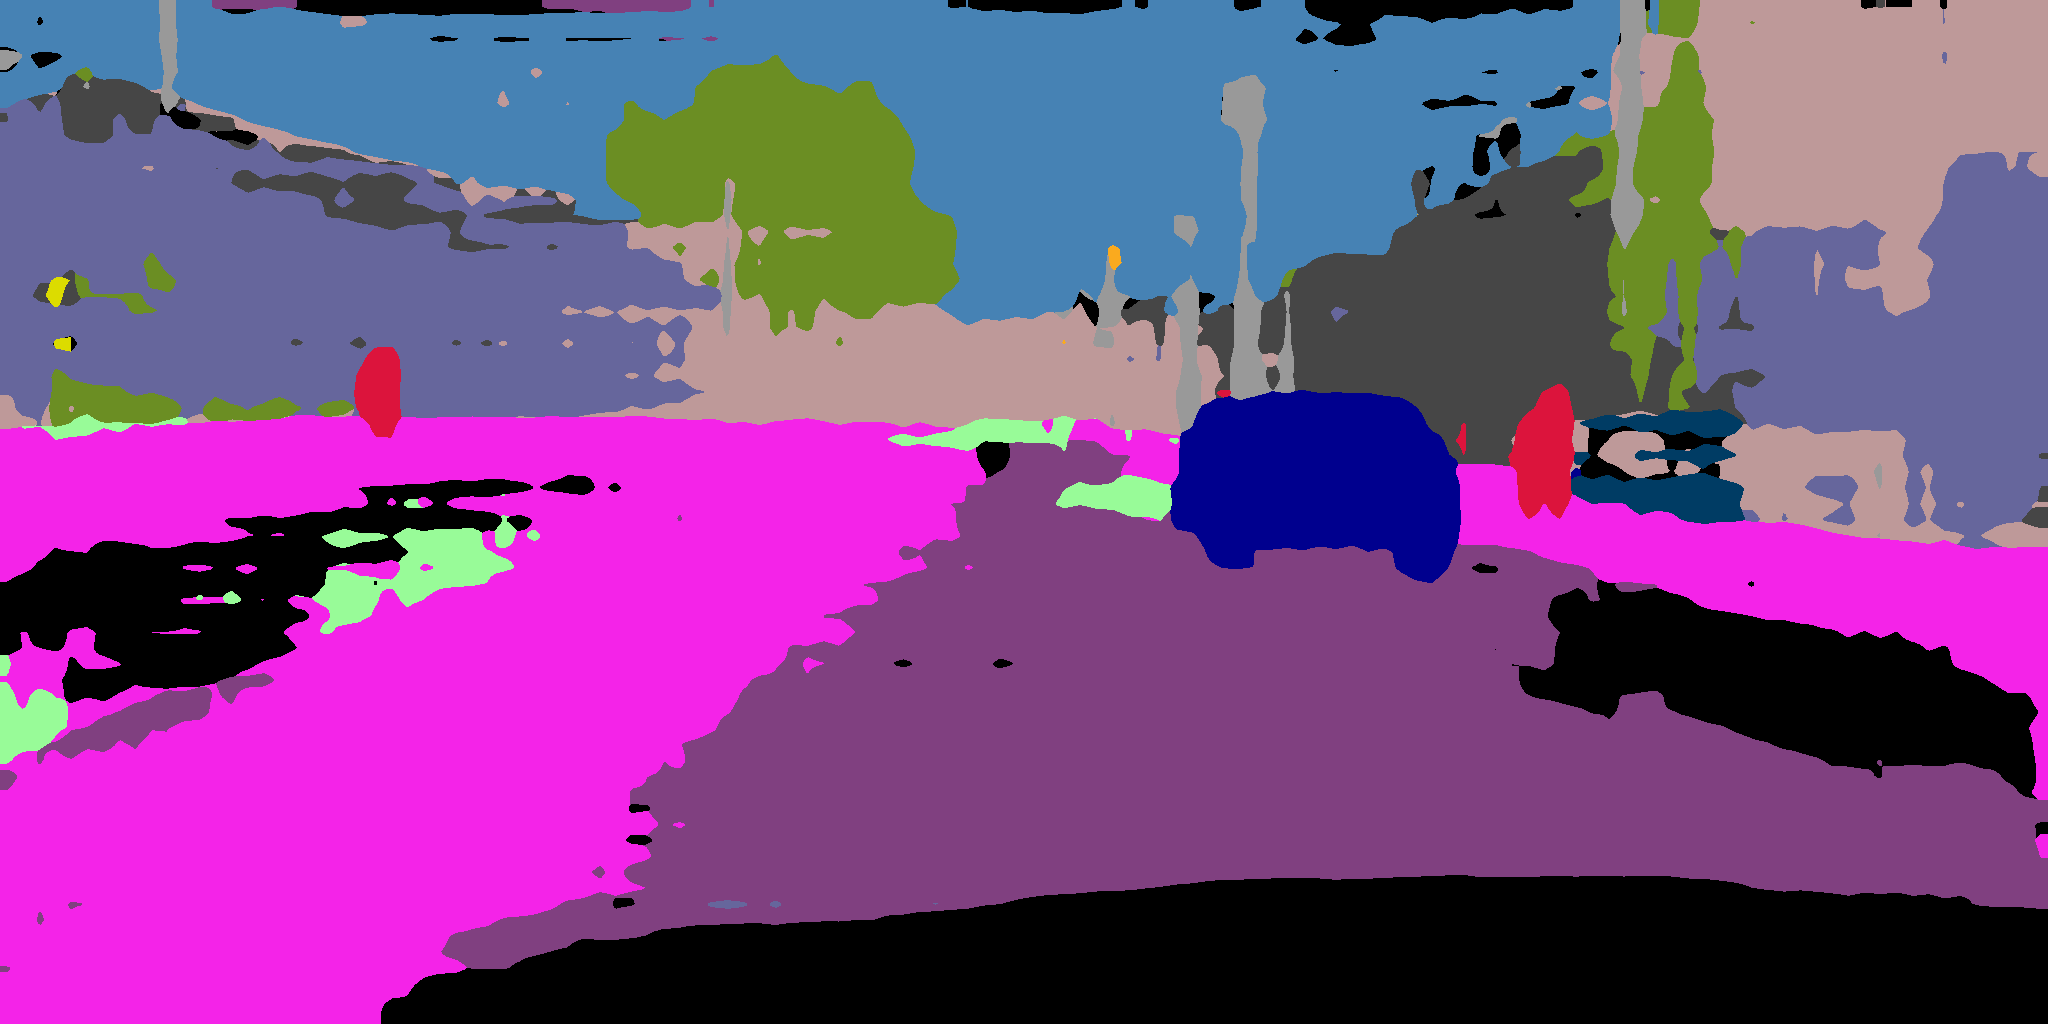
\includegraphics[width=\textwidth]{images/evaluation/SG-GAN_pred_labels.png}
		\end{minipage} \\
		%\multicolumn{2}{c}{} \\
		\multicolumn{1}{c}{} & (translated) Image & (predicted) Labelmap
	\end{tabular} 
	\caption{Ground Truth image and corresponding Ground Truth labelmap from the GTA dataset (top) and the images translated by the different techniques (left side) with their corresponding predicted labelmaps (right side)}
	\label{table:results_qual}
	\bigskip
	\centering
	\begin{tabular}{cccccccccccccccccccc}
		\raisebox{-.25\height}{\textcolor{black}{\rule{0.5cm}{0.5cm}}} &
		\raisebox{-.25\height}{\textcolor{purple}{\rule{0.5cm}{0.5cm}}} &
		\raisebox{-.25\height}{\textcolor{lightpurple}{\rule{0.5cm}{0.5cm}}} &
		\raisebox{-.25\height}{\textcolor{grey}{\rule{0.5cm}{0.5cm}}} &
		\raisebox{-.25\height}{\textcolor{bluepurple}{\rule{0.5cm}{0.5cm}}} &
		\raisebox{-.25\height}{\textcolor{darkerskin}{\rule{0.5cm}{0.5cm}}} &
		\raisebox{-.25\height}{\textcolor{grey2}{\rule{0.5cm}{0.5cm}}} &
		\raisebox{-.25\height}{\textcolor{orange}{\rule{0.5cm}{0.5cm}}} &
		\raisebox{-.25\height}{\textcolor{lightgreen}{\rule{0.5cm}{0.5cm}}} &
		\raisebox{-.25\height}{\textcolor{green}{\rule{0.5cm}{0.5cm}}} &
		\raisebox{-.25\height}{\textcolor{brightgreen}{\rule{0.5cm}{0.5cm}}} &
		\raisebox{-.25\height}{\textcolor{blue}{\rule{0.5cm}{0.5cm}}} &
		\raisebox{-.25\height}{\textcolor{red}{\rule{0.5cm}{0.5cm}}} &
		\raisebox{-.25\height}{\textcolor{fullred}{\rule{0.5cm}{0.5cm}}} &
		\raisebox{-.25\height}{\textcolor{darkblue}{\rule{0.5cm}{0.5cm}}} &
		\raisebox{-.25\height}{\textcolor{blueblack}{\rule{0.5cm}{0.5cm}}} &
		\raisebox{-.25\height}{\textcolor{paleblue}{\rule{0.5cm}{0.5cm}}} &
		\raisebox{-.25\height}{\textcolor{palegreenblue}{\rule{0.5cm}{0.5cm}}} &
		\raisebox{-.25\height}{\textcolor{brightblue}{\rule{0.5cm}{0.5cm}}} &
		\raisebox{-.25\height}{\textcolor{brownred}{\rule{0.5cm}{0.5cm}}} \\
		\rotatebox[origin=r]{90}{void} & \rotatebox[origin=r]{90}{road} & \rotatebox[origin=r]{90}{sidewalk} & \rotatebox[origin=r]{90}{building} & \rotatebox[origin=r]{90}{wall} & \rotatebox[origin=r]{90}{fence} & \rotatebox[origin=r]{90}{pole} & \rotatebox[origin=r]{90}{traffic light} & \rotatebox[origin=r]{90}{traffic sign} & \rotatebox[origin=r]{90}{vegetation} & \rotatebox[origin=r]{90}{terrain} & \rotatebox[origin=r]{90}{sky} & \rotatebox[origin=r]{90}{person} & \rotatebox[origin=r]{90}{rider} & \rotatebox[origin=r]{90}{car} & \rotatebox[origin=r]{90}{truck} & \rotatebox[origin=r]{90}{bus} & \rotatebox[origin=r]{90}{train} & \rotatebox[origin=r]{90}{motorcycle} & \rotatebox[origin=r]{90}{bicycle}
	\end{tabular} 
	\caption{Color coding of semantic classes used in semantic segmentation labelmaps.}
	\label{table:semseg_colors}
	\setlength\tabcolsep{6pt}
\end{table}


\newpage

\section{Discussion}
CyCADA performed best on average for both category and class Scores in this comparison. From the translated images used in this comparison it looks like CyCADA was able to smoothen textures more than the other methods giving them a more realistic look. This is especially obvious when looking at the ``flat'' category scores where it improves semantic segmentation by as much as $15.4\%$. The untranslated GTA images having the best scores for human, sky and object categories is probably due to noise and artifacts generated by the adaptation techniques. This results in reduced details for instances of the human category which is generally already smaller (pixel-wise) than the other categories. SG-GAN creates a lot of noise into the sky which makes correct prediction of sky labels a lot harder for the DeepLabv3 model. SG-GAN performing best for cars and busses might be due to generating distinct pixels around semantic boundaries which may result in better distinction between instances of cars and busses far in the background and their surroundings. The ``glow'' is especially visible between the sky and its neighboring semantic classes. This might be the reason for SG-GAN to perform best for traffic signs as they are easier to seperate from the background. Overall, the results are not as expected. All of the techniques compared in this work show in their corresponding papers that they improve the performance of semantic segmentation models compared to unadapted images for GTA to Cityscapes domain adaptation. This is not the case here. This is probably due to the models used in this work not being the ones the authors actually used in their works. Therefore, it can't be ensured that they were trained the way the authors describe which may result in the decrease in average performance for CycleGAN and SG-GAN. 
